%% 
%% Copyright 2007-2020 Elsevier Ltd
%% 
%% This file is part of the 'Elsarticle Bundle'.
%% ---------------------------------------------
%%
%% It may be distributed under the conditions of the LaTeX Project Public
%% License, either version 1.2 of this license or (at your option) any
%% later version.  The latest version of this license is in
%%    http://www.latex-project.org/lppl.txt
%% and version 1.2 or later is part of all distributions of LaTeX
%% version 1999/12/01 or later.
%% 
%% The list of all files belonging to the 'Elsarticle Bundle' is
%% given in the file `manifest.txt'.
%% 
%% Template article for Elsevier's document class `elsarticle'
%% with harvard style bibliographic references

\documentclass[preprint,12pt]{elsarticle}

%% Use the option review to obtain double line spacing
%% \documentclass[preprint,review,12pt]{elsarticle}

%% Use the options 1p,twocolumn; 3p; 3p,twocolumn; 5p; or 5p,twocolumn
%% for a journal layout:
%% \documentclass[final,1p,times]{elsarticle}
%% \documentclass[final,1p,times,twocolumn]{elsarticle}
%% \documentclass[final,3p,times]{elsarticle}
%% \documentclass[final,3p,times,twocolumn]{elsarticle}
%% \documentclass[final,5p,times]{elsarticle}
%% \documentclass[final,5p,times,twocolumn]{elsarticle}

%% For including figures, graphicx.sty has been loaded in
%% elsarticle.cls. If you prefer to use the old commands
%% please give \usepackage{epsfig}

%% The amssymb package provides various useful mathematical symbols
\usepackage{amssymb}
%% The amsthm package provides extended theorem environments
%% \usepackage{amsthm}

%% The lineno packages adds line numbers. Start line numbering with
%% \begin{linenumbers}, end it with \end{linenumbers}. Or switch it on
%% for the whole article with \linenumbers.
%% \usepackage{lineno}

\usepackage[table]{xcolor}
\usepackage{booktabs}
\usepackage{todonotes}


\journal{Information Processing \ Management}

\begin{document}

\begin{frontmatter}

%% Title, authors and addresses

%% use the tnoteref command within \title for footnotes;
%% use the tnotetext command for theassociated footnote;
%% use the fnref command within \author or \address for footnotes;
%% use the fntext command for theassociated footnote;
%% use the corref command within \author for corresponding author footnotes;
%% use the cortext command for theassociated footnote;
%% use the ead command for the email address,
%% and the form \ead[url] for the home page:
%% \title{Title\tnoteref{label1}}
%% \tnotetext[label1]{}
%% \author{Name\corref{cor1}\fnref{label2}}
%% \ead{email address}
%% \ead[url]{home page}
%% \fntext[label2]{}
%% \cortext[cor1]{}
%% \affiliation{organization={},
%%             addressline={},
%%             city={},
%%             postcode={},
%%             state={},
%%             country={}}
%% \fntext[label3]{}

\title{We need to beat namespotting, no idea how}

%% use optional labels to link authors explicitly to addresses:
%% \author[label1,label2]{}
%% \affiliation[label1]{organization={},
%%             addressline={},
%%             city={},
%%             postcode={},
%%             state={},
%%             country={}}
%%
%% \affiliation[label2]{organization={},
%%             addressline={},
%%             city={},
%%             postcode={},
%%             state={},
%%             country={}}

\author{Us}

\affiliation{organization={},%Department and Organization
            addressline={}, 
            city={},
            postcode={}, 
            state={},
            country={}}

\begin{abstract}
Abstract goes here. 

\end{abstract}

%%Graphical abstract
\begin{graphicalabstract}
Not sure what graphical abstract is supposed to be, but it goes here. 
\end{graphicalabstract}

%%Research highlights
\begin{highlights}
\item Research highlight 1
\item Research highlight 2
\end{highlights}

\begin{keyword}
 keyword \sep keyword


\PACS PACScode \sep PACScode

\MSC MSCcode \sep MSCcode
%% or \MSC[2008] code \sep code (2000 is the default)

\end{keyword}

\end{frontmatter}


\tableofcontents

%% \linenumbers

%% main text

\section{Data analysis}\label{sec{analysis}}

\subsection{Exploration and data}\label{subsec:data-and-exploration}



For the duration of the project we selected 486 Reddit users\todo{how?} and tracked
their activity (with some breaks resulting from API restrictions and
technical issues, which were mostly sorted out in the observation
period), starting on 2020-03-09, beginning the intervention period on
2020-07-08, leading to a further observation period starting on
2020-09-09 and ending on 2020-11-20. The time series of attacks observed
and of interventions conducted can be inspected in Figure
\ref{fig:periodsPlot}, along with a quick search for weekly patterns.
Some of the users turned out to be bots, a few ceased to be active
during the experiment (with no strong reason to think this happened due
to them receiving an intervention) and a few received treatment of two
different types by accident (we relied on multiple volunteers and such
mistakes were likely to happen). Ultimately, in the time series data, we
ended up with data on 440 users.



\begin{figure}
\begin{center}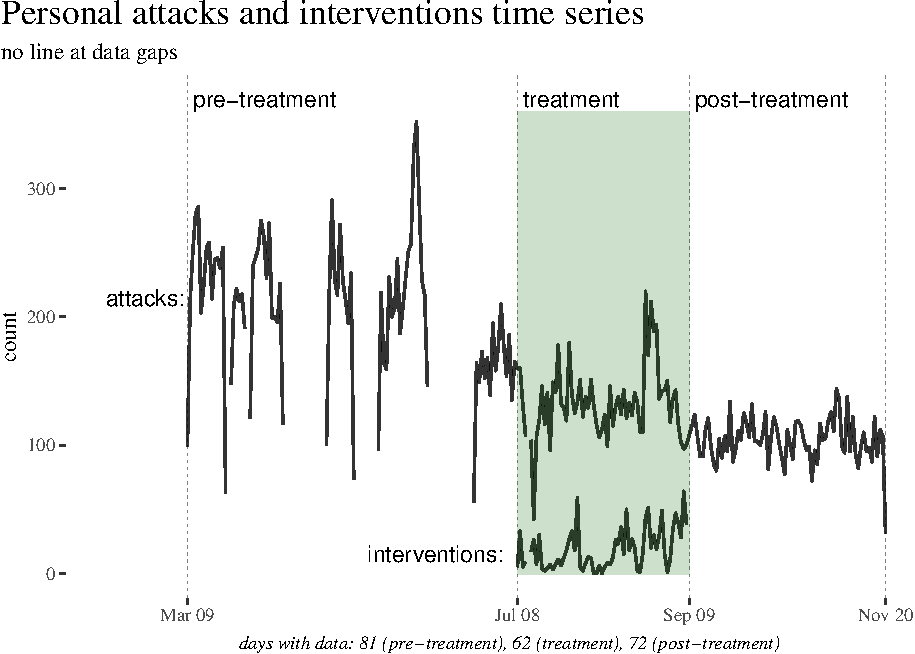
\includegraphics[width=0.88\linewidth]{figures/periodsPlot-1} 

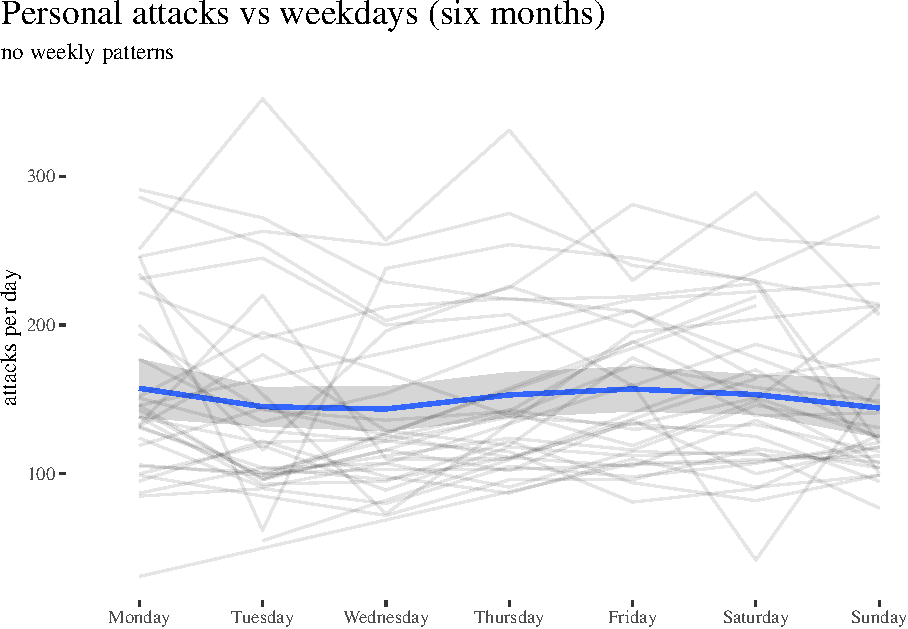
\includegraphics[width=0.88\linewidth]{figures/periodsPlot-2} \end{center}
\caption{Daily sums of attacks and interventions throughout the three experimental periods, with GAM smoothing (left) and daily attack sums from all  weeks in the experimental period plotted against week days (right)---no pattern seems to arise.}
\label{fig:periodsPlot}
\end{figure}


We analyzed the data from three perspectives: we used the daily data to
(1) build seven time series models estimating the impact of individual
interventions at lags 1-7 days, and (2) to study the impact of the
cumulative number of total interventions received as the experiment
progressed, and (3) we used aggregated data to run a long term
before-and after analysis, comparing the summarized aggression levels
before and after the intervention period.



Before we move to the analysis, let us inspect the data. First, at the
aggregated level, the data involve the variables listed in Table
\ref{tab:baaVars}.\footnote{Further variables were defined in terms of those, in particular, we will be predicting \textsf{AdiffS} which is the standardized difference  \textsf{AA}-\textsf{AB}, and \textsf{AdiffS}, which is the standardized difference \textsf{CA}-\textsf{CB}.The  standardized variables are systematically named  $\langle$variable\char`_name$\rangle$S.} The distribution of \textsf{IC} in the treatment groups is visualized in
Figure \ref{fig:interventionsDistro}. Note that the distributions are
somewhat different, even though the total intervention counts are
similar. The issue is discussed in Section XXXXX.\todo{add ref}


\vspace{1mm}
\footnotesize

\normalsize

\begin{table}
\centering
\begin{tabular}{ll}
\toprule
variable  explanation\\
\midrule
\cellcolor{gray!6}{AB}  \cellcolor{gray!6}{attacks before (pre-treatment)}\\
AD  attacks during (the treatment period)\\
\cellcolor{gray!6}{AA}  \cellcolor{gray!6}{attacks after (post-treatment)}\\
CB  comments before\\
\cellcolor{gray!6}{CD}  \cellcolor{gray!6}{comments during}\\
CA  comments after\\
\cellcolor{gray!6}{group}  \cellcolor{gray!6}{treatment group}\\
IC  intervention count\\
\bottomrule
\end{tabular}

\caption{Variables involved in the before-and-after analysis.}
\label{tab:baaVars}
\end{table}



\begin{figure}

\begin{center}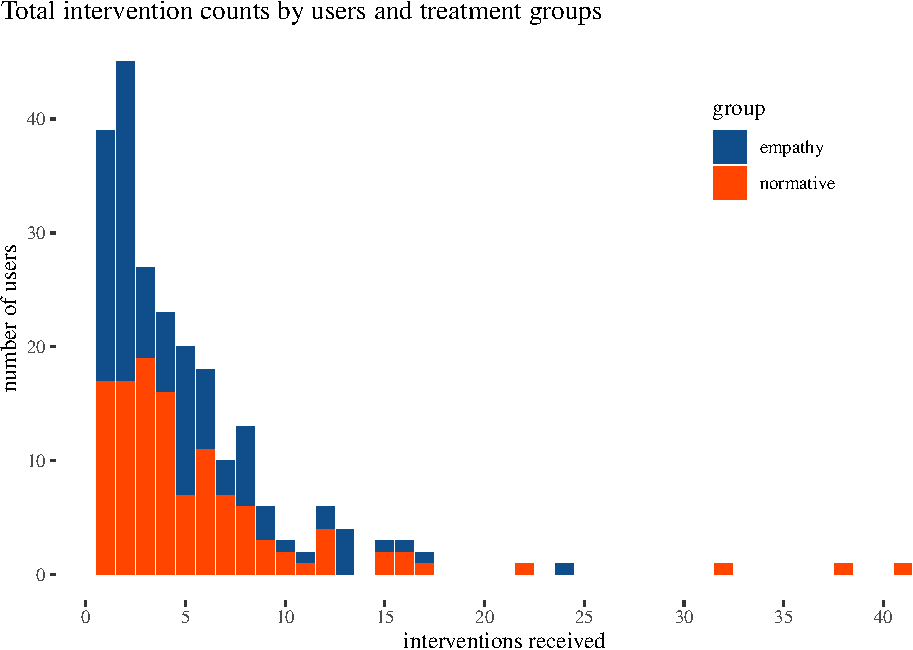
\includegraphics[width=.88\linewidth]{figures/interventionsDistroPlot-1} \end{center}
\caption{Distribution of daily interventions (by treatment group).}
\label{fig:interventionsDistro}
\end{figure}

Second, in the distribution of standardized difference in attacks, the
peaks of distributions are shifted a bit between the groups, with lowest
median for the normative group, but the differences seem minor (Figure
\ref{fig:violJoint}). This might suggest no impact of the interventions.
This conclusion would be too hasty, as the impact of other predictor
variables and interactions involved can mask actual associations.




\begin{figure}

\begin{center}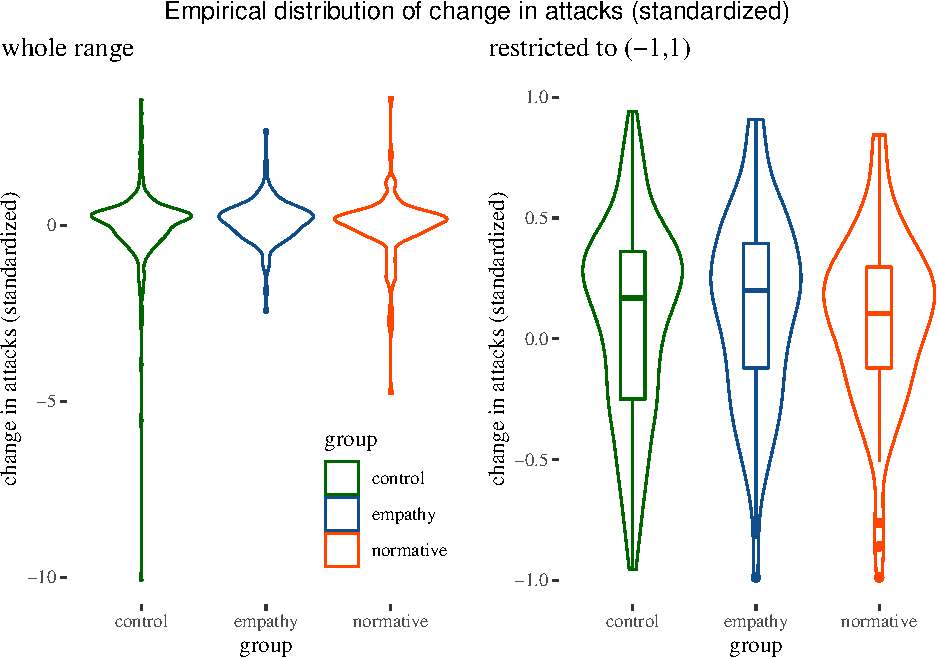
\includegraphics[width=1\linewidth]{figures/violJoint-1} \end{center}
\caption{Empirical distribution of change in attacks (by treatment group).}
\label{fig:violJoint}
\end{figure}

To see how this masking can occur, let us inspect changes in attacks
against intervention counts. It turns out that restricting attention to
various aggression levels in the before period results in fairly strong
changes to the regression lines (Figure \ref{fig:linearShift}). This
suggests we should keep an eye out for interactions with aggression
before in the analysis, and that the initial comparison of means or
medians between groups might be misleading if the effects in different
volume groups are different and to some extent cancel each other.



\begin{figure}

\begin{center}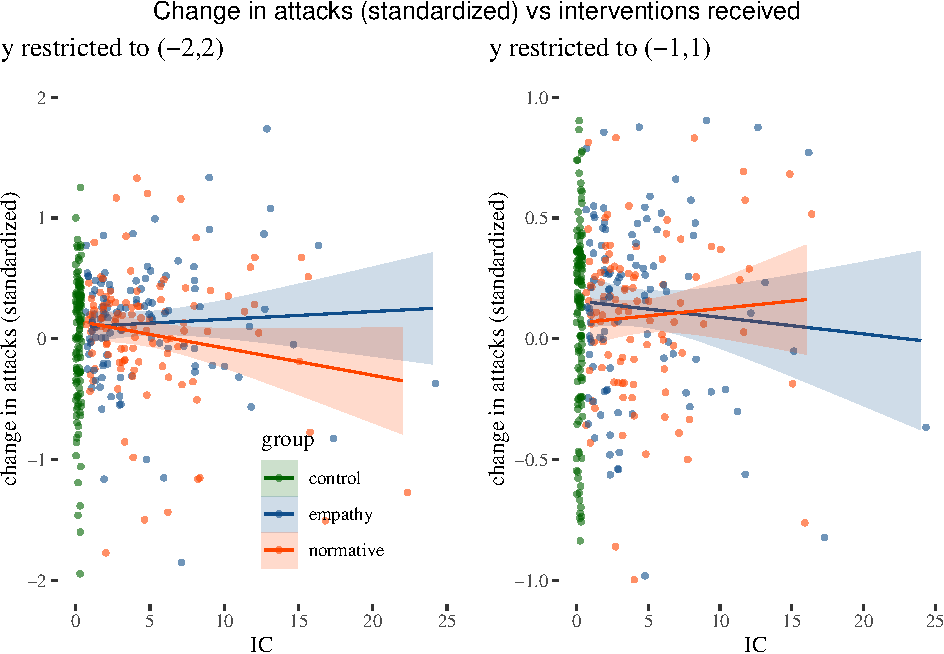
\includegraphics[width=1\linewidth]{figures/fig:linearShift-1} \end{center}
\caption{Change in attacks vs the number of interventions received by treatment group, jittered with  linear smoothing.}
\label{fig:linearShift}
\end{figure}

\normalsize

Further insights, undermining the initial impression suggested by Figure
\ref{fig:violJoint}, can be obtained by visualizing individual time
series. Figure \ref{fig:tsVis} contains six fairly typical examples.






\begin{figure}

\begin{center}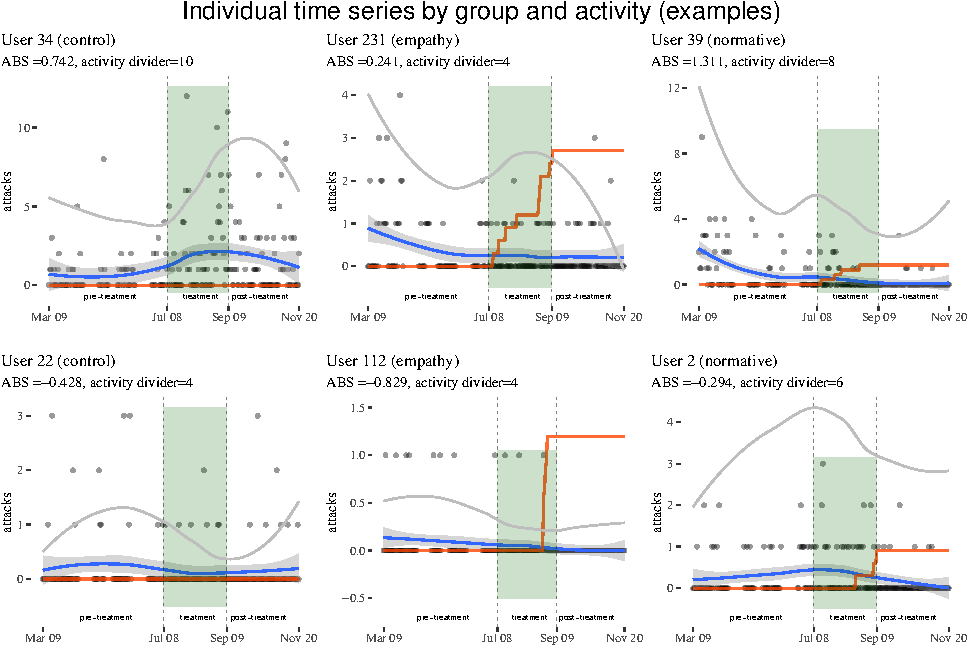
\includegraphics[width=1\linewidth]{figures/fig:tsVisPlot6-1} \end{center}
\caption{Examples of individual time series. Black points are attacks (smoothed in blue), red lines represent the cumulative number of interventions received (lag 3) divided by 10, gray lines represent overall activity level divided by a variable divider listed in the subtitle. Divisions introduced for visual comparability of general trends.}
\label{fig:tsVis}
\end{figure}

\normalsize

The general phenomenon is that while in the control group attacks tend
not to diminish, unless activity itself diminishes, they tend to
diminish in the normative group (although the more aggressive the user
is, the less of an impact can be observed), and in the empathetic group
if the user is not very aggressive. Of course, visualization of
individual cases (which the reader might suspect to be cherry-picked) is
no replacement for statistical analysis, to which we will now move.



\subsection{Causal thinking, choice of variables and
models}\label{subsec:causal-thinking-choice-of-variables-and-models}

First, we inspect correlations between predictors to avoid multicolinearity, as highly correlated predictors do not improve predictive performance and artificially inflate uncertainty in their corresponding coefficients in the models. We then develop
a plausible causal model of the situation (Figure
\ref{fig:correlations}). It turns out that to avoid multicolinearity we
cannot condition on CDS if we condition on CAS or CBS. Similarly, for
the time series data, since activity levels in particular day slices are
correlated, it will not be useful to condition on more than one
auto-regressive element (and since the predictive power is the highest
for lag 1 with no discoverable weekly patterns, we will not go further
than lag 1).

To choose the right variables to condition (or not condition) on to
identify the causal effect of the interventions, we need to think about
the causal structure of the problem. Comments during (the intervention period) impact attacks
during, which trigger interventions. Unmeasured user features cause
comments before (the intervention period), which impact attacks before directly. Comments during
(their impact on ADS is already included) impact attacks during directly
and comments after, which impact attacks after and attacks after
directly. Intervention count impacts attacks after and comments after.
The same directions of impact are included for intervention type.
Finally, comments through time are connected causally, and so are
attacks. The structure for the time series data is analogous, except now
instead of before and after, we have multiple daily indices.



\begin{figure}

\begin{center}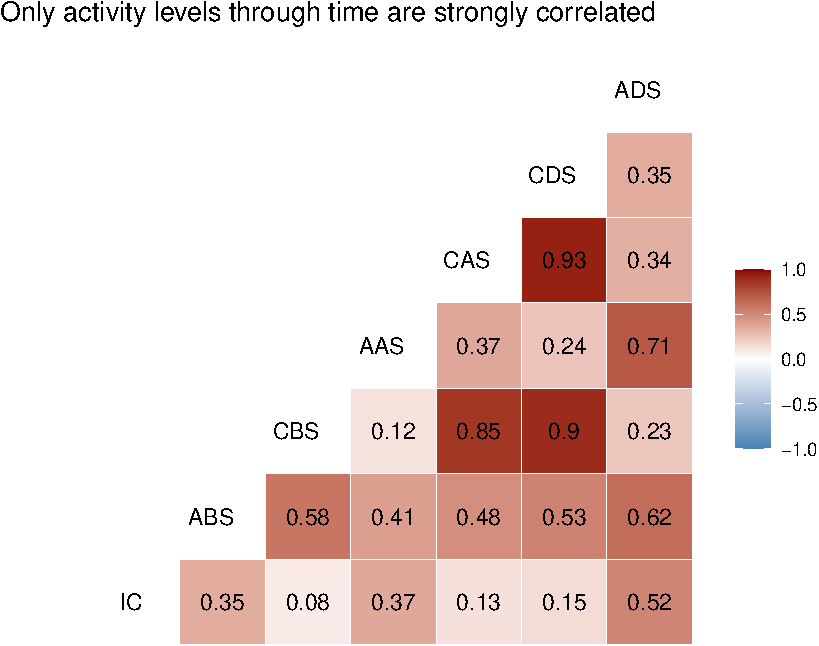
\includegraphics[width=0.48\linewidth]{figures/correlations-1} 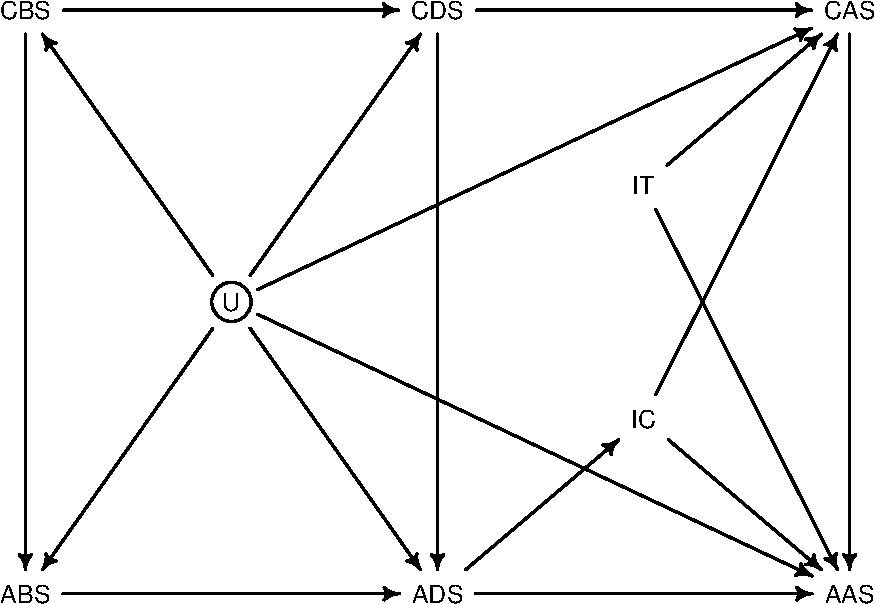
\includegraphics[width=0.48\linewidth]{figures/correlations-2} \end{center}

\caption{Correlations between predictors (left) and a plausible causal model (right) used in the before-and-after analysis.}
\label{fig:correlations}
\end{figure}



What do we learn from causal considerations? \textsf{IT} has no backdoor
paths, but \textsf{IC} does, so we need to make sure these are closed to
avoid including spurious correlations in our analysis. There are in fact
65 different paths from \textsf{IC} to \textsf{AAC}. Crucially, all
backdoor paths go through \textsf{ADS}, which then becomes either a fork
or a pipe, so all backdoor paths can be closed by conditioning on
\textsf{ADS}. Moreover there is only one directed indirect path, it goes
through \textsf{CAS}, so we should not condition on \textsf{CAS} if we
are to identify total causal effect of \textsf{IC} on attacks, including
the impact mediated by its impact on comments. We might be interested in
the direct effect of \textsf{IC} and \textsf{IT} on \textsf{AAS}, but
then we also need to block indirect causal paths from the intervention
to the outcome. For such an evaluation we would need to also condition
on \textsf{CAS} and block all backdoor paths from \textsf{CAS} to
\textsf{AAS}. This, however, given the causal model, cannot be achieved,
as it would required conditioning on unobserved user features. That is,
we do not think direct causal effect is identifiable.

Analogous considerations apply to the time series model for the total
impact of individual interventions received exactly \(k\) days before
(in our case, \(k\in \{1, \dots, 7\}\)). The situation, however, is
somewhat different for the impact of the total number of cumulative
interventions received so far. The trouble is, for example, that if a
user received so far a number of interventions until yesterday, some of
them had been received before yesterday and those had already impacted
their aggression level yesterday. In other words, conditioning on lagged
attacks leads to the post-treatment bias and should be
avoided.\footnote{In fact, in the aggregated data analysis, we will be predicting the standardized difference between attacks before and after (\textsf{ADiffS}), and the standardized difference between comments, before and after (\textsf{CDiffS}), but the general points about the nodes involved apply also to defined nodes.  As already discussed, we do not include \textsf{CDS} because of its strong correlation with \textsf{CBS}. We also do not condition on \textsf{ABS} when modeling \textsf{ADiffS} (or on \textsf{CBS} when modeling \textsf{CDiffS})---not only because it has a pretty strong correlation with another predictor (\textsf{ADS}), but rather also because it is used to define the output variable. In such a set-up, it is clear that a model including \textsf{ABS} would have better predictive power, but since a definitional connection is present, thinking that its inclusion in the model tells us something about causality  would be misled.}

Otherwise, it's open season for the other variables and interactions
between them, and our decision to include or exclude them in the model
will be guided by information-theoretic criterion of predictive power, whose more detailed explanation is  included in the appendix, the so-called
Widely Acceptable Information Criterion:
\[
\mathsf{WAIC(y, \Theta)}  = -2 (\mathsf{lppd} - \overbrace{\sum_i var_\theta \mathsf{log} p (y_i \vert \theta)}^{\mathsf{penalty}})
\]
We also use  posterior predictive checks in cases in which the likelihood
functions used by the models to be compared are different and
information-theoretic calculations might be misleading. In such cases we
investigated the ratio of actual observations included in the 50\% and
in the 89\% posterior predictive distribution, and the models for which
higher ratios were observed in both were selected (no case of diverging
evaluation for the two criteria has been observed).

In our model building we used the \textsf{rethinking} package,
except for the cumulative impact time series models, where it becomes
computationally unfeasible, in which case we built models in
\textsf{Rstan} directly. Moreover, for the time series analysis we will
build hierarchical Bayesian models which tend to have around
\(u \times 2p + 2p\) parameters (we will explain later why), which means
that for 440 users our final model with interaction with six predictors
would have \(440 \times 12 + 12 = 5292\) parameters, and 
have to be trained on daily data for 7 variables collected for six months. The
building of such a model on a modern computer takes days. Since in
reaching this model we needed to build multiple somewhat simpler models
or models with different structures and test their performance, model
selection on the full data set was unfeasible. That is, in the time
series analysis in model selection at each step we compared models
(sometimes built with quadratic approximation) with respect to three
independent samples for \(40, 60\) and \(60\) users. We made the
decision only if a given model structure performed better on all these
subsets (which was usually the case, so the model selection criteria
gave us pretty robust answers). For the most complicated model of the
impact of cumulative number of interventions, building a single model
for the whole data set was not computationally feasible (computation
time does not increase linearly with the number of users included in the
dataset), so we randomly split the dataset 
and provided results for the subgrous---the results were not very divergent and the highest posterior density intervals were not very wide.





For the time series, the model that the procedure led us to is as follows (see the appendix for a detailed explanation of how this model has been reached):

\footnotesize

\begin{center}
\begin{tabular}{c}
$\mathsf{attacks}_i  \sim  \mathsf{NegativeBinomial}(\lambda_i, \phi_{\mathsf{userID[i]}} ) $\\
$log(\lambda_i)  =  l_{\mathsf{userID[i]}} +
                  a_{\mathsf{userID[i]}} \times \mathsf{attacksL1} +
                  c_{\mathsf{userID[i]}} \times \mathsf{act} + $\\
$                   + 
       i1control_{\mathsf{userID[i]}} \times  \mathsf{control} \times \mathsf{intL1D}  +$ \\$         +  i1emp_{\mathsf{userID[i]}} \times  \mathsf{emp} \times \mathsf{intL1D}  +$ \\$
              +  i1norm_{\mathsf{userID[i]}} \times  \mathsf{norm} \times \mathsf{intL1D}
                          $\\ 
$  l_{\mathsf{userID[i]}}   \sim \textsf{Norm}(\bar{l}, \bar{\sigma_l}) $\\
$  a_{\mathsf{userID[i]}}  \sim \textsf{Norm}(\bar{a}, \bar{\sigma_a}) $\\
$  c_{\mathsf{userID[i]}}  \sim \textsf{Norm}(\bar{c}, \bar{\sigma_c}) $\\
 $ i1control_{\mathsf{userID[i]}}  \sim  \textsf{Norm}(i1controlOverall,\bar{\sigma_{i1}})$ \\
$   i1emp_{\mathsf{userID[i]}}  \sim  \textsf{Norm}(i1empOverall, \bar{\sigma_{i1}})$\\  
 $ i1norm_{\mathsf{userID[i]}}   \sim  
     \textsf{Norm}(i1normOverall, \bar{\sigma_{i1}})$\\
$     i1controlOverall  \sim  \textsf{Norm}(0,.2)$\\
$    i1empOverall   \sim  \textsf{Norm}(0,.2) $\\
$    i1normOverall   \sim  \textsf{Norm}(0,.2) $\\
$    \bar{\lambda}   \sim  \textsf{Norm}(.00001, 2.5) $\\
$    \bar{\sigma_l}  \sim  \mathsf{Exp}(1.5)$\\
$    \bar{a}  \sim \textsf{Norm}(0, .2) $\\
$    \bar{\sigma_a}  \sim  \mathsf{Exp}(5) $\\
$    \bar{c}  \sim  \mathsf{Norm}(0, .2)$\\
$    \bar{\sigma_c}  \sim \mathsf{Exp}(5) $\\
$    \bar{\sigma_{i1}}  \sim  \mathsf{Exp}(5)
$
\end{tabular}
\end{center}

\normalsize



\noindent This might seem somewhat confusing, so let us disentangle this maze:

\begin{itemize}
\item Each user has their own baseline aggression level, $l_{\mathsf{userID[i]}}$. \item However, these individual aggression levels are not disconnected, they come from a distribution themselves, $\textsf{Norm}(\bar{l}, \bar{\sigma_l})$. $\bar{l}$ is the mean baseline aggression level for the whole population, and $\bar{\sigma_l}$ is the standard deviation of this distribution. These general parameters are to be estimated along with the individual ones.
\item Then  there are individual auto regression coefficients     $a_{\mathsf{userID[i]}}$, which capture the correlation between  yesterday's attacks with today's attacks, so to speak. These also come from a general distribution \linebreak  $\textsf{Norm}(\bar{a}, \bar{\sigma_a})$, with its own general parameters to be estimated.
\item Next, there are individual user's coefficients connecting the user's activity on a given day with their aggression on the same day,  $c_{\mathsf{userID[i]}}$, all coming from a general distribution $\textsf{Norm}(\bar{c}, \bar{\sigma_c})$ whose parameters are also to be estimated.
\item For any particular treatment group, say, empathy, we have a user level coefficient $i1emp_{\mathsf{userID[i]}}$, which is activated if the user is in the empathy group (that is, we multiply by the indicator variable $\mathsf{emp}$) and then applied to the number of interventions received the day before (lag 1). Similarly for the two other groups. These user-level parameters come from the distribution $\textsf{Norm}(i1empOverall, \bar{\sigma_{i1}})$, whose parameters are to be estimated.
\item Finally, prior predictive check was used to choose priors for the general coefficients. 
\end{itemize}




For the impact of the cumulative number of interventions (we will only
use lag 3 for reasons that will become clear), since the range of values
of the predictor is wider, for computational feasibility we further
needed to restrict coefficients to lie between -3 and 2, but these
values are not plausible values of the parameters anyway
(\(exp(-3) \approx 0.04\) and \(exp(2) \approx 7.38\)). The model for
the cumulative impact was tested with and without interaction with
overall aggression in the before period, without the use of attacks on a
given day (as already explained, to avoid the post-treatment bias). The
two relevant options   are:



\footnotesize


\begin{center}
\begin{tabular}{c}
$log(\lambda_i)  =  l_{\mathsf{userID[i]}}  + c_{\mathsf{userID[i]}} \times \mathsf{act} + 
      ic3control_{\mathsf{userID[i]}} \times  \mathsf{control} \times \mathsf{intCL3D}  + $\\$  + 
            ic3emp_{\mathsf{userID[i]}} \times  \mathsf{emp} \times \mathsf{intCL3D}  + $\\  
    $  ic3norm_{\mathsf{userID[i]}} \times  \mathsf{norm} \times \mathsf{intCL3D}$\\
$log(\lambda_i)  =  l_{\mathsf{userID[i]}}  + c_{\mathsf{userID[i]}} \times  act + $\\$  + 
      ic3control_{\mathsf{userID[i]}} \times   \mathsf{control} \times  \mathsf{intCL3D}  + $\\$  + icabst3control_{\mathsf{userID[i]}} \times   \mathsf{control} \times  \mathsf{intCL3D} \times  \mathsf{abst} + $\\ 
        \end{tabular}
\end{center}

\begin{center}
\begin{tabular}{c}
  $log(\lambda_i)  =  l_{\mathsf{userID[i]}}  + c_{\mathsf{userID[i]}} \times \mathsf{act} + 
      ic3control_{\mathsf{userID[i]}} \times  \mathsf{control} \times \mathsf{intCL3D}  + $\\ $ +    ic3emp_{\mathsf{userID[i]}} \times   \mathsf{emp} \times  \mathsf{intCL3D}  + $\\$  + icabst3emp_{\mathsf{userID[i]}} \times   \mathsf{emp} \times  \mathsf{intCL3D}  \times  \mathsf{abst} + $\\ $ +
        ic3norm_{\mathsf{userID[i]}}] \times   \mathsf{norm} \times  \mathsf{intCL3D} + $\\ $ + icabst3norm_{\mathsf{userID[i]}} \times   \mathsf{norm} \times  \mathsf{intCL3D} \times  \mathsf{abst} 
        $
        \end{tabular}
\end{center}


\normalsize

The models employing the second formula were superior in performance. It
is not surprising that once attacks on a given day were removed from
predictor, the overall aggression levels in the before period became
predictive. The price to pay, however, is that now to obtain a
user-specific multiplicative interpretation of the impact of cumulative
interventions, we need to put the two elements together while
multiplying one by the user's overall aggression and only then
exponentiate, that is we need to inspect, for instance,
\(exp(ic3emp_{\mathsf{userID[i]}} + icabst3emp_{\mathsf{userID[i]}} \times \mathsf{abst}[i])\),
instead of simply looking at \(exp(ic3emp_{\mathsf{userID[i]}})\).






Finally, in the before-and-after analysis, we put aside the time series
element, look at aggregated counts before and after the treatment
period, thus obtaining a more of a long-term effect analysis. Moreover,
this time we standardize counts, obtaining continuous variables and
employing normal distribution in the likelihoods, thus also making sure
the overall results are robust under a spectrum of modeling choices. We
build and compared multiple additive models where the outcome variable
is normally distributed around the predicted mean, which is a linear
function of predictors (possibly with interactions). Our general criteria
led to the model whose specification is as follows (we also selected
regularizing prior parameters using prior predictive checks to avoid
unreasonably narrow overall prior distributions, see the appendix for a longer explanation):


\footnotesize


\begin{center}
\begin{tabular}{c}
$\mathsf{AdiffS}  \sim \textsf{Norm}(\mu, \sigma)$\\
$\mu_i  = \alpha + \beta_{\mathsf{ADS}}[\mathsf{group}_i]\times \mathsf{ADS} + \beta_{\mathsf{group}_i}  +
 \beta_{\mathsf{IC}}[\mathsf{group}_i]\times \mathsf{IC} + $\\
$  + \beta_{\mathsf{ADSIC}}\times \mathsf{ADS} \times \mathsf{IC} + \beta_{\mathsf{CBS}}[\mathsf{group}_i] \times \mathsf{CBS}$\\
$ \alpha  \sim \textsf{Norm}(0,.3)$\\
$\beta_{\mathsf{ADS}}[\mathsf{group}_i]  \sim \textsf{Norm}(0,.3)$\\
$\beta_{\mathsf{group}_i}  \sim \textsf{Norm}(0,.3)$\\
$\beta_{\mathsf{IC}}[\mathsf{group}_i]  \sim \textsf{Norm}(0,.3)$\\
$ \beta_{\mathsf{ADSIC}}  \sim \textsf{Norm}(0,.3)$\\
$ \beta_{\mathsf{CBS}}[\mathsf{group}_i] \sim \textsf{Norm}(0,.3)$\\
\end{tabular}
\end{center}

\normalsize 

That is, we take the resulting mean to be the result of the general
average (\(\alpha\)) and the impact of the following coefficients:
group-specific coefficient for \textsf{ADS}, group coefficient,
group-specific coefficient for \textsf{IC}, interaction coefficient for
\textsf{ADS} and \textsf{IC}, and group-specific coefficient for
\textsf{CBS}. This is plausible \emph{prima facie}, as which group a
user belongs to might have impact on how the number of attacks during
the treatment are related to the number of attacks after, the role of
the intervention count, and the role of comments before. Moreover, the
levels of aggressive behavior displayed by the user during treatment
might have impact on the role played by the intervention count.









\subsection{Results}\label{subsec:resultss}


\subsubsection{Interventions on a given
day}\label{subsubsec:interventions-on-a-given-day}




We built seven separate models for the impact of interventions \(k\)
days ago, \(1\leq k \leq 7\). In Figure \ref{fig:dailyResults} we
visualize the results for the three groups, with jitter based on user
aggression in the before period.


\begin{figure}

\begin{center}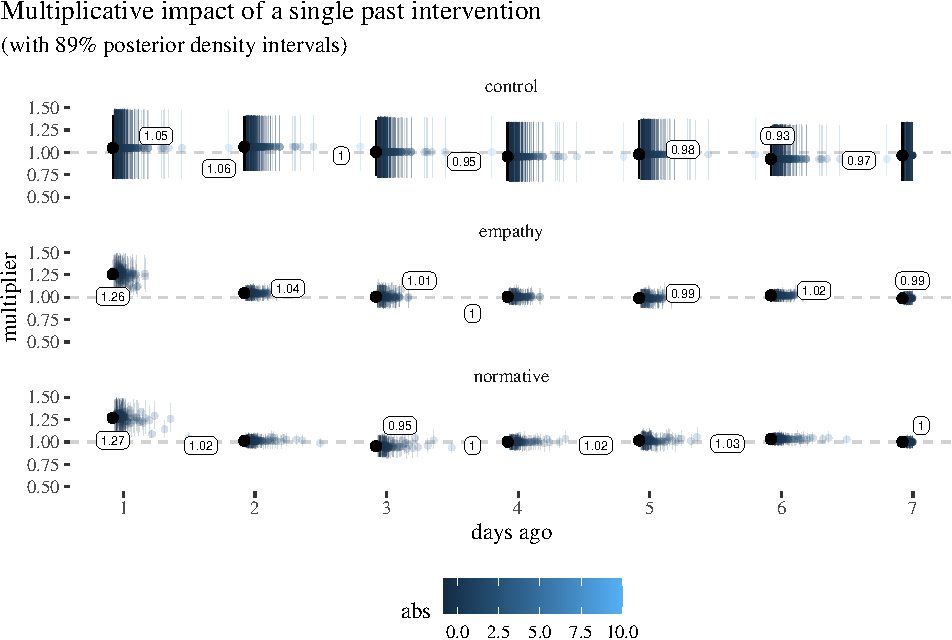
\includegraphics[width=1\linewidth]{ figures/fig:dailyResultsPlot-1} \end{center}
\caption{Impact of interventions received lag $1\leq k \leq 7$ on attacks on a given day. High-level coefficients are pictured in black.}
\label{fig:dailyResults}
\end{figure}

Notice that in short term, interventions actually increase aggression
the next day (even taking the user's yesterday's aggression and today's
activity in consideration). The effect, however, quickly wears off.


\subsubsection{Cumulative sum of
interventions}\label{subsubsec:cumulative-sum-of-interventions}




In our analysis of the effect of the cumulative number of interventions
received so far, however, we intend separate this short-term effect from
the long-term effect. To achieve this, we lag the cumulative
interventions variable by 3, so that we're giving the user the minimal
number of days needed for the short-term effect to wane. The individual
users' multiplicative impact coefficients are visualized in Figure
\ref{fig:cumulativeResultsPlot}.


\begin{figure}

\begin{center}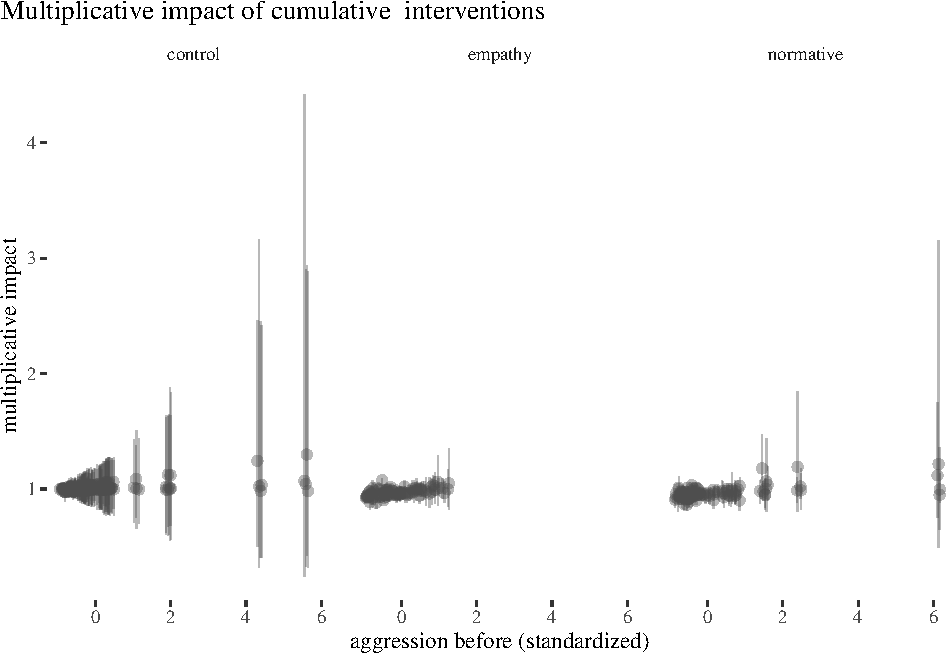
\includegraphics[width=.8\linewidth]{ figures/fig:cumulativeResultsPlot-1} 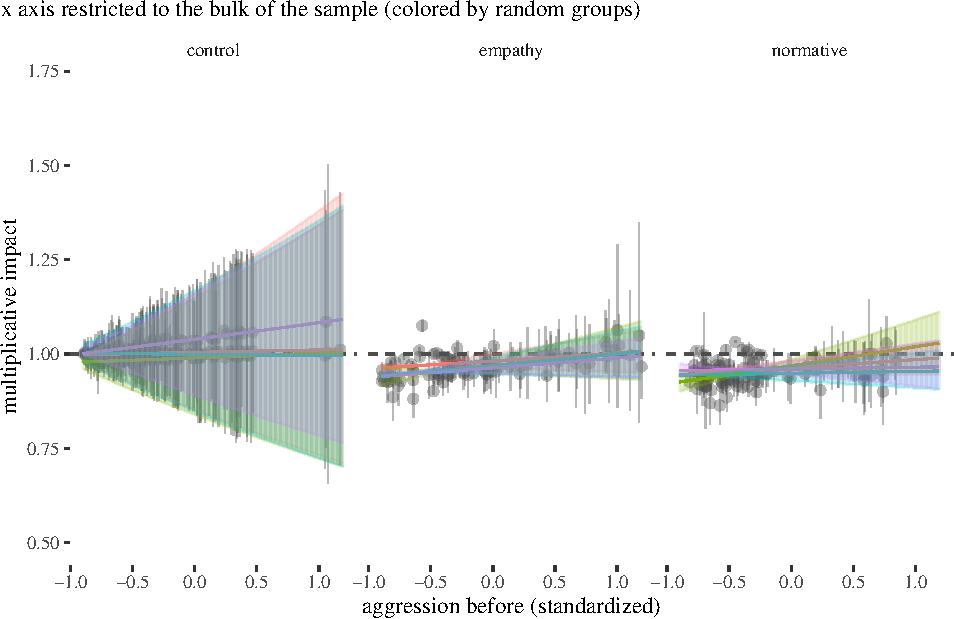
\includegraphics[width=.8\linewidth]{ figures/fig:cumulativeResultsPlot-2} \end{center}
\caption{Multiplicative impact of cumulative interventions lag 3 on attacks. Individual users' coefficents only, full range (top), and with attention restricted to the bulk of the sample. Sub-sample coefficients depend on aggression and are represented as lines, colored by sub-sample. Note low number and high uncertainty for highly aggressive users, which motivate the restriction of the $x$ axis for inspection.}
\label{fig:cumulativeResultsPlot}
\end{figure}

\normalsize

The efficiency of normative interventions seems overall higher, except
for low-aggression users, for which empathetic interventions might be
equally or more useful. Importantly, linear extrapolation to extreme
values might be misleading, so let us inspect on what happens with the
general level multiplicative coefficients at the levels of aggression
which are actually quite common, that is, at the 1st, 2nd and 3rd
quartile (with respect to \(\mathsf{abst}\)). This indicates that for
the bulk of the sample the impact of cumulative interventions has been
negative, slightly more so on users with lower aggression levels.






\begin{figure}

\begin{center}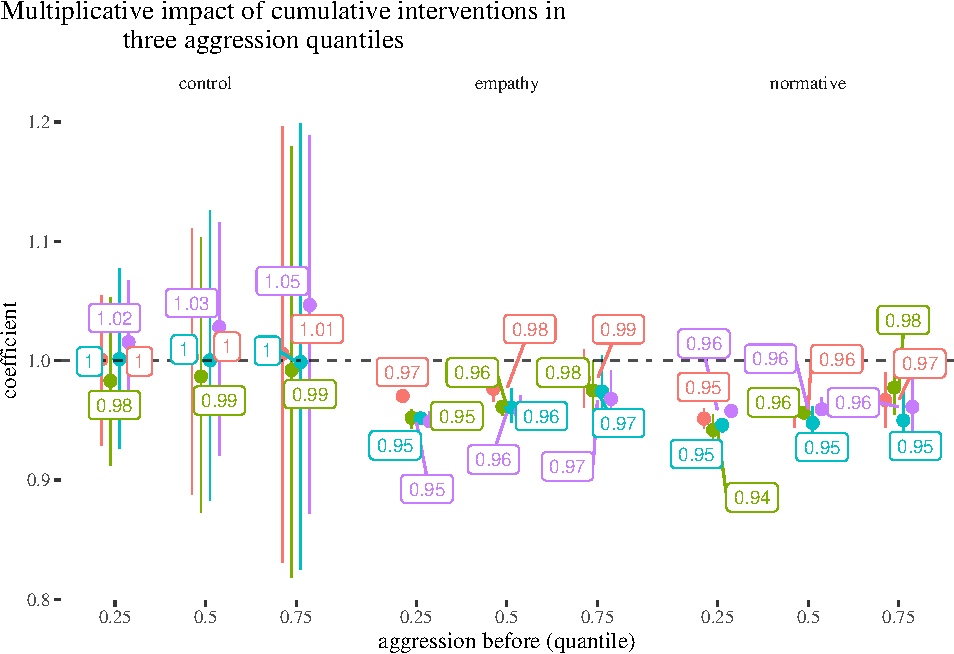
\includegraphics[width=1\linewidth]{ figures/fig:cumulativeResultsGeenralPlot-1} \end{center}
\caption{Multiplicative impact of cumulative interventions lag 3 on attacks. General level coefficents only, in three quantiles (.25, .5, .75). Colored by sub-sample.}
\label{fig:cumulativeResultsGeneralPlot}
\end{figure}


\subsubsection{Long term before/after
analysis}\label{subsubsec:long-term-beforeafter-analysis}

The general problem with interpreting  models of this complexity involving
interaction is  that coefficients are not directly interpretable. For this reason, it is better
to plot predicted effects for various combinations of predictors. In the
construction of the plots we rely on the following:

\begin{itemize}
\item The values \textsf{ADS} range from -.67 to 10, with approximately 30\% below -.5, around 80\% below .3, and around 95\% below 1.7, so we use these three settings of this variable in our visualizations. 

\item The values \textsf{CBS} range from -.82 to 18.3, with approximately 30\% below -.4, around 80\% below .3, and around 95\% below 1.3, so we use these three settings of this variable in our visualizations. 


\end{itemize}

% \begin{figure}
% \begin{center}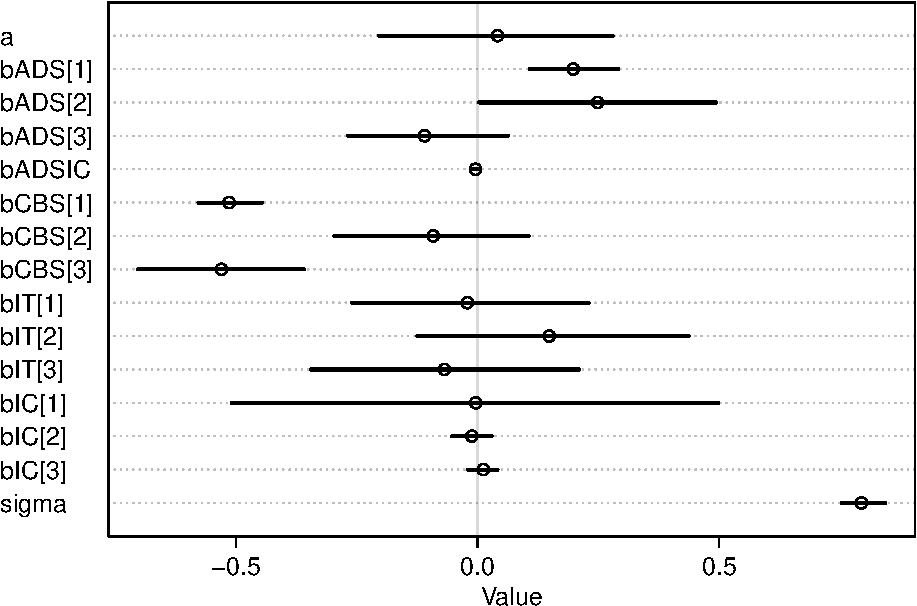
\includegraphics[width=1\linewidth]{ figures/unnamed-chunk-3-1} \end{center}
% \caption{The final model coefficients.}
% \label{fig:coeffs}
% \end{figure}




Grouped before-and-after predicted change of attacks by the levels we
just listed are visualized in Figure \ref{fig:predictedChange}. For more clarity, let's inspect predicted contrasts, here understood as
distances from the control group mean, by activity level, first versus
CBS (comments before, standardized, Figure \ref{fig:ContrastCBS}), then
versus ADS (attacks during, standardized, Figure \ref{fig:ContrastADS}).


\begin{figure}

\begin{center}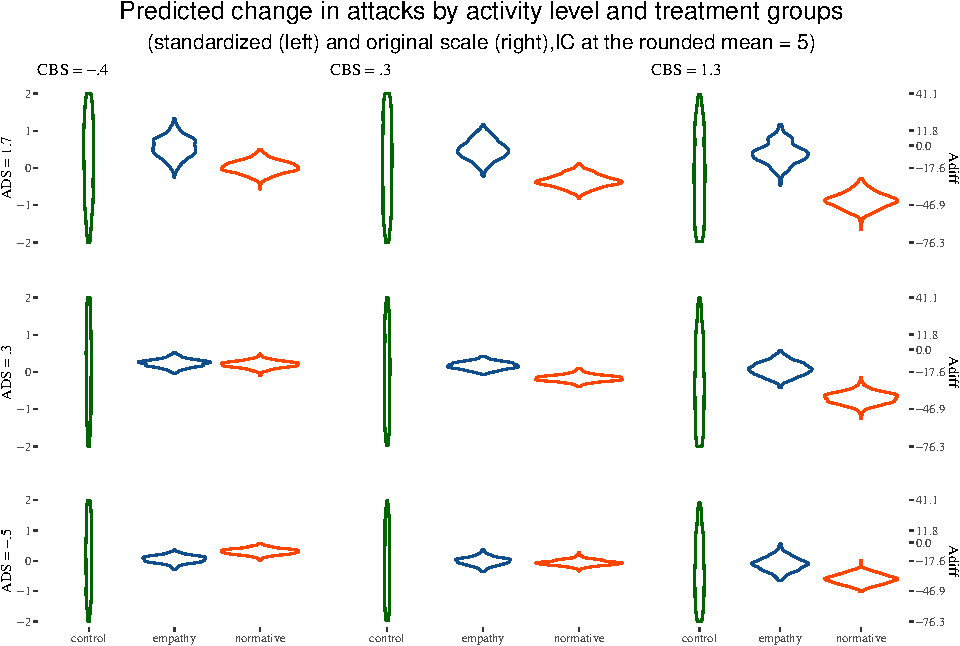
\includegraphics[width=1\linewidth]{ figures/unnamed-chunk-5-1} \end{center}
\caption{Predicted change in attacks, depending on user’s activity level
(CBS: comments before, standardized) and how aggressive overall they
were (ADS: attacks during, standardized). The more aggressive and active
the users, the higher the attacks drop in the normative group, slight drop
correlated with emotive interventions for not too active users.}
\label{fig:predictedChange}
\end{figure}







\begin{figure}

\begin{center}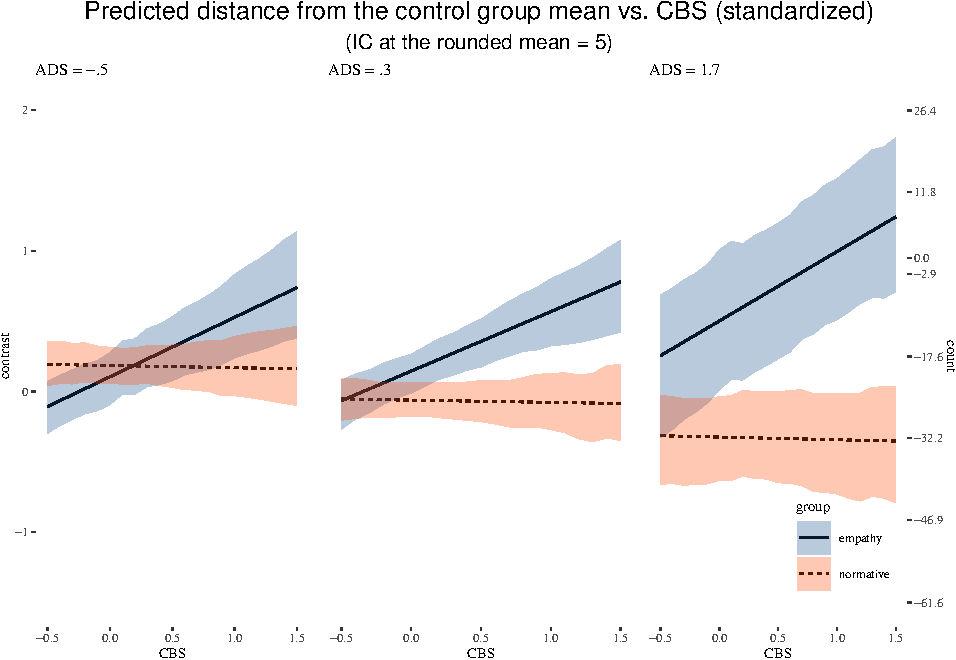
\includegraphics[width=1\linewidth]{ figures/unnamed-chunk-7-1} \end{center}
\caption{Predicted contrasts (difference in attacks as compared to the control group)
for the two treatment groups vs activity before the treatment. Notice that
empathetic interventions correlated with decreased attacks for less active
users, but performed worse than normative interventions for more active
users. Normative interventions, in contrast, seem to have better impact on
 more active users.}
\label{fig:ContrastCBS}
\end{figure}




\begin{figure}

\begin{center}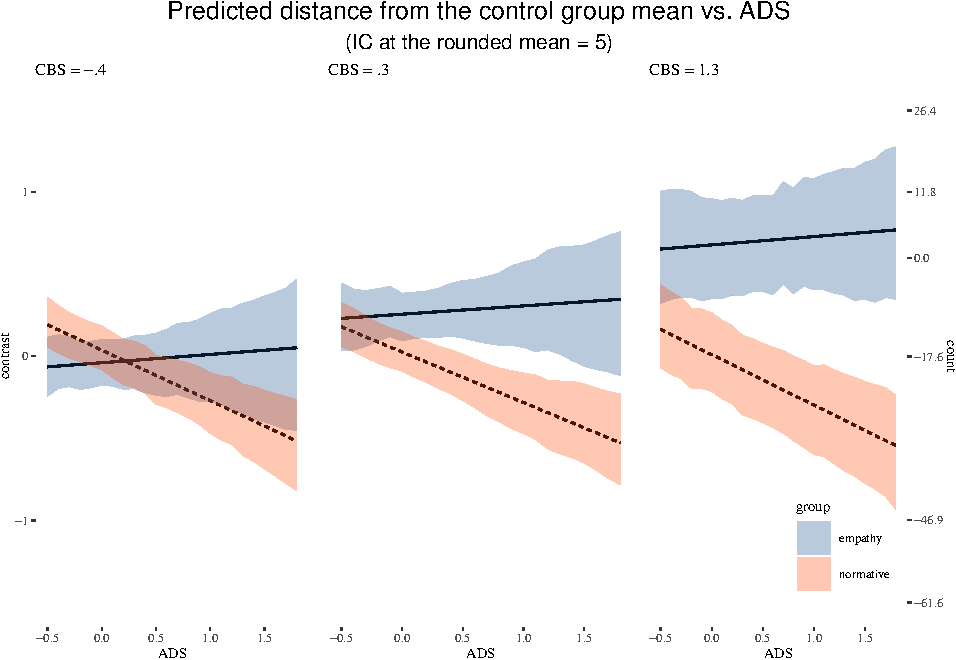
\includegraphics[width=1\linewidth]{ figures/unnamed-chunk-9-1} \end{center}
\caption{Predicted contrasts (difference in attacks as compared to the control group)
for the two treatment groups vs aggression during the treatment period.
Notice that empathetic interventions correlated with decreased attacks for
less aggressive users, but performed worse than normative interventions for
more aggressive users. Normative interventions, in contrast, seem to have
better impact on  more aggressive users.}
\label{fig:ContrastADS}
\end{figure}




Now, let's inspect the impact of intervention counts by treatment type
by looking at contrasts (distances from the control group mean) with
89\% HPDIs by IC (intervention count). Notice the predicted effect of IC
is weaker than group membership, so for visibility the \(y\)-axis has a
smaller range. Also, not enough data was available to reliably estimate
uncertainty for IC above 20, hence the restriction on the \(x\)-axis
(already at lower values, lack of estimates is visible for the more
extreme settings).





\begin{figure}

\begin{center}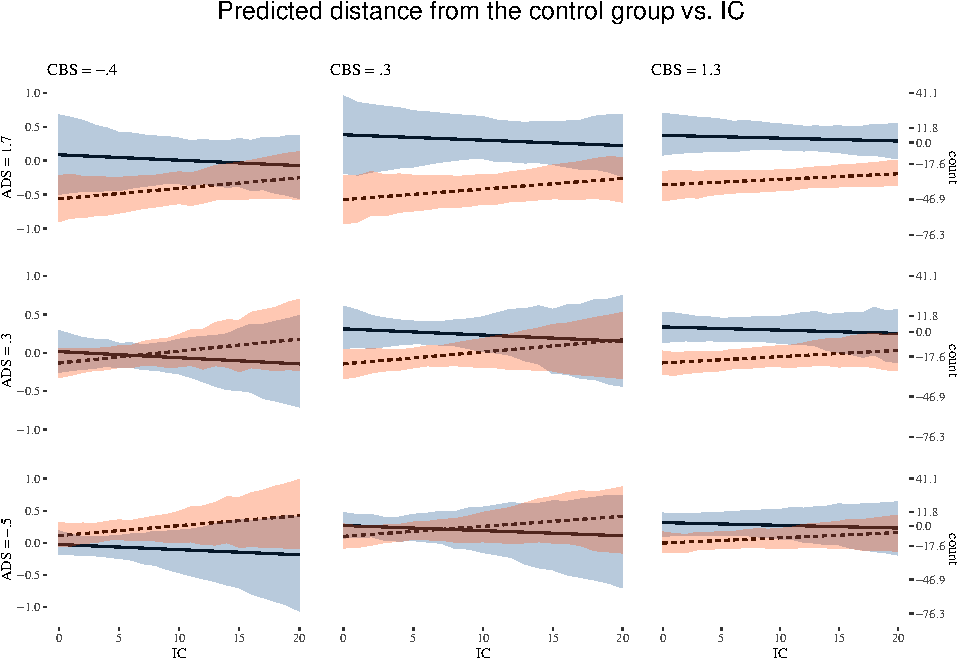
\includegraphics[width=1\linewidth]{ figures/visICPlot-1} \end{center}
\caption{Contrasts (change in attacks as compared to the control group) vs the number
of interventions received. Note that repeating empathetic interventions
correlates with decreased attacks, while repeating normative interventions
is counterproductive.}
\label{fig:ContrastsIC}
\end{figure}



\section{Discussion}














\section{Volunteer engagement and impact of competitions}


\subsection{The challenge of keeping volunteers engaged}


\subsection{Volunteer activity  data analysis}


The winning model, given our model selection method, is specified as
follows:


\footnotesize


\begin{center}
\begin{tabular}{c}
$\mathsf{interventions} \sim \mathsf{NegativeBinomial} (\lambda,\phi) $\\
$log(\lambda) = l_\mathsf{volunteerID[i]} + enth_\mathsf{ volunteerID[i]} \times \mathsf{daysOfProject} + comp_\mathsf{volunteerID[i]} \times \mathsf{competition}$\\  
$l_\mathsf{ volunteerID[i] }  \sim \mathsf{Norm}(lbar,lsigmabar) $\\
$lbar \sim \mathsf{Norm}(2, .9)$\\
$lsigmabar, enthsigmabar, compsigmabar \sim  \mathsf{Exp}(.5) $\\
$enth _\mathsf{ volunteerID[i] }  \sim \mathsf{Norm}(enthbar, enthsigmabar)$\\
$comp_\mathsf{ volunteerID[i] } \sim \mathsf{Norm}(compbar, compsigmabar) $\\
$enthbar, compbar \sim  \mathsf{Norm}(0, .3)$\\
$ \phi =  puser_\mathsf{ volunteerID[i] } $ \\
$ puser_\mathsf{ volunteerID[i] } \sim \mathsf{Exp}(1)$
\end{tabular}
\end{center}


\normalsize


Intuitively, volunteer interventions are assumed to have negative
binomial distribution around their own expected value \(\lambda\) and
individualized dispersion parameters \(\phi\). On each day each a user
has their own daily expected value, which is determined by the following
factors:

\begin{itemize}
\item First, there's user's individual baseline activity for the whole treatment period, $l_\mathsf{ volunteerID[i] }$.
\item next, each user has their own dispersion parameter,  $puser_\mathsf{ volunteerID[i] }$.
\item then, there is (usually dwindling) enthusiasm: the impact of time on that user, $enth_\mathsf{volunteerID[i]} $ to be (after exponentiation) multiplied by the number of days that have passed since the experiment started,
\item finally, we have the impact that the presence of competitions made on a user, $comp_\mathsf{ volunteerID[i] }$, which (after exponentiation) becomes the activity multiplier to be applied during competitions only.
\end{itemize}

\noindent Moreover, the model is hierarchical: the individual level
parameters are drawn from distributions whose parameters are in turn to
be estimated as well. Thus, \(lbar\) is the overall baseline for the
whole group, \(enthbar\) is the overall estimated group enthusiasm
coefficient, and \(compbar\) is the overall estimated competition impact
coefficient (all of them come with their own nuisance sigma parameters).

\noindent All of these parameters are given priors in a manner analogous
to the introduction of priors for the other time series models, as
explained in the appendix.\footnote{Interestingly, if we are interested
  in the causal effect of competitions, we should not use an
  auto-regressive predictor. If we auto-regress on a lag in the
  \([1,7]\) range, for some days we will be conditioning on
  interventions conducted during the same competition, which will
  already contain some information about the impact of that competition.
  In other words, auto-regression with short lags would lead to
  post-treatment bias. On the other hand, auto-regression with longer
  lags would either lead to dropping a lot of data in the beginning
  (where lagged information is not available), or degenerate the
  analysis by using 0s for missing lagged values in a long initial
  period. All this without much gain, as we have already inspected null
  models with auto-regression with large lags and they do not lead to
  performance improvement.}

Raw data and daily means are illustrated in Figure
\ref{fig:volunteersBasic}, and the individualized totals with the key
coefficients based on the trained model are illustrated in Figure
\ref{fig:volunteersModel}.

\begin{figure}

\begin{center}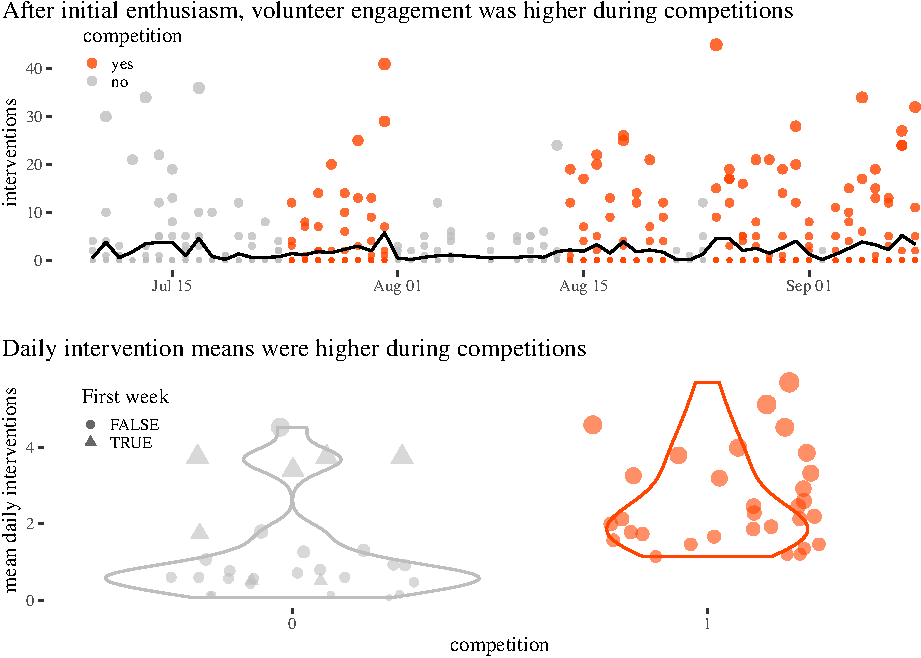
\includegraphics[width=1\linewidth]{figures/fig:volunteersBasic5-1} \end{center}
\caption{Daily individual voilunteer intervention counts accross time with competition periods marked (top) and daily group intervention means grouped by whether a competition was ongoing (bottom). Note most of high means in the non-competition period are in the first week.}
\label{fig:volunteersBasic}
\end{figure}

\begin{figure}

\begin{center}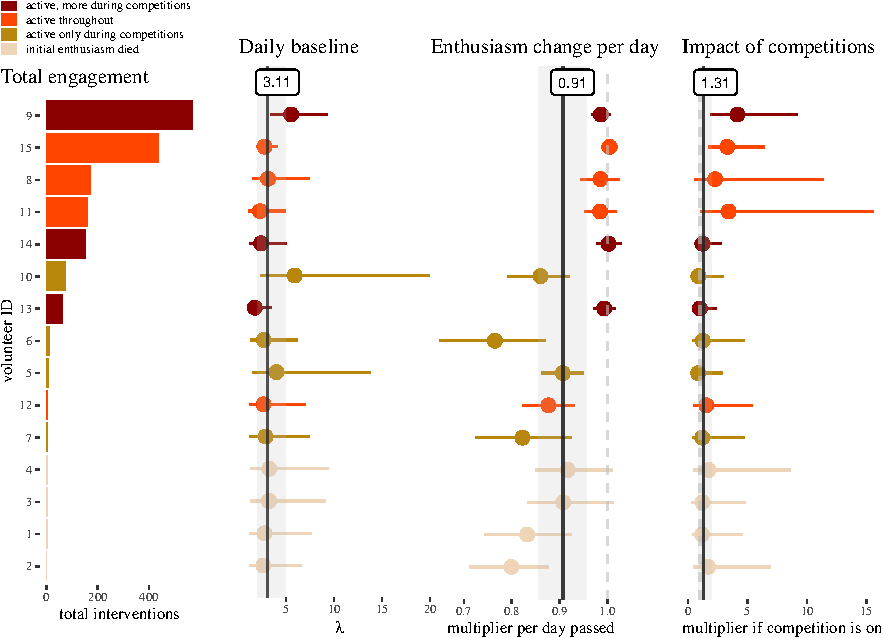
\includegraphics[width=1\linewidth,angle=90]{figures/fig:volunteersModel17-1} \end{center}
\caption{Volunteer total engagement with their daily baseline and multipliers for enthusiasm and impact of competition. Pointranges represent individual level coefficients, group coefficients are represented by black lines with shaded 89\% HPDI areas.}
\label{fig:volunteersModel}
\end{figure}
















%% The Appendices part is started with the command \appendix;
%% appendix sections are then done as normal sections
\appendix


\section{Explanation of WAIC}

 Let  $y$ be the observations and $\Theta$  a posterior distribution.
First, log-pointwise-predictive-density is defined by:
\[
\mathsf{lppd}(y, \Theta)  = \sum_i log\frac{1}{S}\sum_s p (y_i\vert \Theta_s)
\]
\noindent where $S$ is the number of samples in the posterior, and $\Theta_s$ 
is the $s$-th combination of sampled parameter values in the posterior distribution. That is, 
for each observation and each combination of 
parameters in the posterior we first compute its density, then 
we take the average density of that observation over all combinations of parameters in the posterior,
and  then take the logarithm. Finally, we sum these values up for all the observations. Crucially, when comparing posterior distributions with respect to the same dataset, \textsf{lppd}s are proportional
 to unbiased estimates of their divergence from the real distribution (note that it is \emph{only} 
 proportional, and for this reason can be used for comparison of distributions 
 only and makes no intuitive sense on its own).  However, \textsf{lppd} always improves
  as the model gets more complex, so for model comparison it makes more sense to use 
 the Widely Applicable Information Criterion (WAIC), which is an approximation of the out-of-sample deviance that converges to the cross-validation approximation in a large sample. It  is defined as
 the log-posterior-predictive-density with an additional
  penalty proportional to the variance in the
  posterior predictions:
\[
\mathsf{WAIC(y, \Theta)} = -2 (\mathsf{lppd} - \overbrace{\sum_i var_\theta \mathsf{log} p (y_i \vert \theta)}^{\mathsf{penalty}})
 \]
\noindent  Thus to construct the penalty, we calculate the variance in log-probabilities for each observation and sum them up. Because of the analogy to Akaike's criterion, the penalty is sometimes called the effective number of parameters, $p_{\mathsf{WAIC}}$. 
How does WAIC compare to other information criteria?  AIC uses MAP estimates instead of the posterior and requires that priors be flat or overwhelmed by the likelihood, and assumes that the posterior distribution is approximately multivariate Gaussian and the sample size is  much greater  than the number of parameters used in the model. Bayesian Information Criterion (BIC) also requires flat priors and uses MAP estimates. WAIC does not make these assumptions, and provides almost exactly the same results as AIC, when AIC’s assumptions are met.


\section{Time series model
selection}\label{sec:time-series-model-selection}

Suppose we are interested in the impact of interventions received \(n\)
days ago. We started with a simple null model that uses the Poisson
distribution, with either uses a single \(\lambda\) for all the users,
or user-specific \(\lambda\)s. The first Bayesian model has the
following structure: 


\footnotesize


\begin{center}
\begin{tabular}{c}
$\mathsf{attacks_i}  \sim  \textsf{Poisson}( \lambda)$\\$
    log(\lambda)   =  l $\\$
    l  \sim  \textsf{Norm}(.05,2.8)$
\end{tabular}
\end{center}

\normalsize

and the user-specific coefficient model had the following structure:


\footnotesize


\begin{center}
\begin{tabular}{c}
$\mathsf{attacks}_i  \sim  \textsf{Poisson}( \lambda_i)$\\$ 
    log(\lambda_i)   =  l_{\mathsf{userID[i]}} $\\$
    l_{\mathsf{userID[i]}}  \sim  \textsf{Norm}(.05,2.8)$
\end{tabular}
\end{center}


\normalsize

The priors were chosen using prior predictive check, so that the 89\%
density intervals reached between 0 and 34, with median around 1. Given
our prior experience with similar user datasets this is a fairly wide
informative prior. The comparison, unsurprisingly, preferred the
user-specific \(\lambda\)s.

Next, we introduced the auto-regressive element, conditioning on
yesterday's attacks. The choice of priors for the auto-regression
coefficient is guided by the visualization (intuitive direct
understanding of the values is made difficult by the fact that the
predictors work on the logarithmic scale) and the fact that larger
values would result in a unreasonably extreme impact of yesterday's
attacks. 



\footnotesize

\begin{center}
\begin{tabular}{c}
$\mathsf{attacks}_i  \sim  \textsf{Poisson}( \lambda_i)$\\$ 
    log(\lambda_i)   =  l_{\mathsf{userID[i]}} + a_{\mathsf{userID[i]}} \times \mathsf{attacksL1}$\\$
    l_{\mathsf{userID[i]}}  \sim  \textsf{Norm}(.05,2.8)$\\$
    a_{\mathsf{userID[i]}}  \sim \textsf{Norm}(0,.2)$
\end{tabular}
\end{center}


\normalsize

Next, we added today's activity level as a predictor, with user-specific
coefficients. Adding activity levels helps. Note also that our priors
taken separately were made more narrow, to preserve the overall width of
the prior predictive distribution (this will be the usual strategy as we
progress). 


\footnotesize


\begin{center}
\begin{tabular}{c}
$\mathsf{attacks}_i   \sim  \textsf{Poisson}( \lambda_i)$\\ 
$    log(\lambda_i)    =  l_{\mathsf{userID[i]}} + a_{\mathsf{userID[i]}} \times \mathsf{attacksL1} + c \times \mathsf{act}$\\ 
$    l_{\mathsf{userID[i]}}   \sim  \textsf{Norm}(.05,2.3)$\\
$    a_{\mathsf{userID[i]}}   \sim \textsf{Norm}(0,.1)$\\
$    c   \sim  \textsf{Norm}(0,.1)$
\end{tabular}
\end{center}



\normalsize

\noindent Unsurprisingly, it helps even more if the
coefficients are user-specific: 



\footnotesize

\begin{center}
\begin{tabular}{c}
$\mathsf{attacks}_i   \sim  \textsf{Poisson}( \lambda_i)$\\ 
 $   log(\lambda_i)    =  l_{\mathsf{userID[i]}} + a_{\mathsf{userID[i]}} \times  \mathsf{attacksL1} + c_{\mathsf{userID[i]}} \times \mathsf{act}$\\ 
  $  l_{\mathsf{userID[i]}}   \sim  \textsf{Norm}(.05,2.3)$\\
 $   a_{\mathsf{userID[i]}}   \sim \textsf{Norm}(0,.1)$\\
$    c_{\mathsf{userID[i]}}   \sim  \textsf{Norm}(0,.1)$
\end{tabular}
\end{center}


\normalsize

A relatively large number of zeros suggests that moving to a
zero-inflated Poisson distribution would be a good idea. It was not, so
the following model structure was tested and abandoned: 



\footnotesize


\begin{center}
\begin{tabular}{c}
$\mathsf{attacks}_i   \sim  \textsf{ZiPoisson}(p, \lambda_i)$\\ 
$    log(\lambda_i)    =  l_{\mathsf{userID[i]}} + a_{\mathsf{userID[i]}}  \times \mathsf{attacksL1} + c_{\mathsf{userID[i]}}  \times \mathsf{act}$\\ 
$    l_{\mathsf{userID[i]}}   \sim  \textsf{Norm}(.05,2.3)$\\
$    a_{\mathsf{userID[i]}}   \sim \textsf{Norm}(0,.1)$\\
$    c_{\mathsf{userID[i]}}   \sim  \textsf{Norm}(0,.1) $\\
$    logit(p)   = \pi$\\
$    \pi   \sim Norm(-1.5,1) $
\end{tabular}
\end{center}

\normalsize


Then we considered the negative binomial distribution, and the addition
of week days as a predictor (both with general and user-level
coefficients). While moving to the negative binomial distribution
resulted in an improvement, adding week days did not improve the model
performance, perhaps because we already conditioned on activity, and
whatever the impact of weekdays was, has been already mediated through
activity (in a sense, we committed a post-treatment bias with respect to
weekdays; but that's fine, we did not really care about the impact of
weekdays).


\footnotesize


\begin{center}
\begin{tabular}{c}
$\mathsf{attacks}_i   \sim  \textsf{NegativeBinomial}(\lambda_i, \phi)$\\ 
$    log(\lambda_i)    =  l_{\mathsf{userID[i]}} + a_{\mathsf{userID[i]}}  \times \mathsf{attacksL1} + c_{\mathsf{userID[i]}}  \times \mathsf{act}$\\ 
$    l_{\mathsf{userID[i]}}   \sim  \textsf{Norm}(.05,2.3)$\\
$    a_{\mathsf{userID[i]}}   \sim \textsf{Norm}(0,.1)$\\
$    c_{\mathsf{userID[i]}}   \sim  \textsf{Norm}(0,.1) $\\
$    \phi  \sim \mathsf{Exp}(1)$\\
\end{tabular}
\end{center}

\begin{center}
\begin{tabular}{c}
$\mathsf{attacks}_i   \sim  \textsf{NegativeBinomial}(\lambda_i, \phi)$\\ 
$    log(\lambda_i)    =  l_{\mathsf{userID[i]}} + a_{\mathsf{userID[i]}}  \times \mathsf{attacksL1} + c_{\mathsf{userID[i]}}  \times \mathsf{act} + w  \times \mathsf{weekday}$\\ 
  $  l_{\mathsf{userID[i]}}   \sim  \textsf{Norm}(.05,2.3)$\\
$    a_{\mathsf{userID[i]}}   \sim \textsf{Norm}(0,.1)$\\
$    c_{\mathsf{userID[i]}}   \sim  \textsf{Norm}(0,.1) $\\
$    w   \sim \textsf{Norm}(0,.1) $\\
$    \phi   \sim \mathsf{Exp}(1)$
\end{tabular}
\end{center}


\begin{center}
\begin{tabular}{c}
$\mathsf{attacks}_i   \sim  \textsf{NegativeBinomial}(\lambda_i, \phi)$\\ 
$    log(\lambda_i)    =  l_{\mathsf{userID[i]}} + a_{\mathsf{userID[i]}}  \times \mathsf{attacksL1} + c_{\mathsf{userID[i]}}  \times \mathsf{act} + w_{\mathsf{userID[i]}}  \times \mathsf{weekday}$\\ 
$    l_{\mathsf{userID[i]}}   \sim  \textsf{Norm}(.05,2.3)$\\
$    a_{\mathsf{userID[i]}}   \sim \textsf{Norm}(0,.1)$\\
$    c_{\mathsf{userID[i]}}   \sim  \textsf{Norm}(0,.1) $\\
$    w_{\mathsf{userID[i]}}   \sim \textsf{Norm}(0,.1) $\\
$   \phi   \sim \mathsf{Exp}(1)$\\
\end{tabular}
\end{center}


\normalsize


We also considered adding overall aggression in before period as a
predictor, but the addition did not lead to improvement. One reason this
is interesting is that interaction of interventions with overall
aggression will turn out to be important for long-term effects.


\footnotesize


\begin{center}
\begin{tabular}{c}
$\mathsf{attacks}_i  \sim  \textsf{NegativeBinomial}(\lambda_i, \phi)$\\ 
$    log(\lambda_i)   =  l_{\mathsf{userID[i]}} + a_{\mathsf{userID[i]}} \times \mathsf{attacksL1} + c_{\mathsf{userID[i]}} \times \mathsf{act} + act + ab_{\mathsf{userID[i]}} \times \textsf{ABS}$\\ 
$    l_{\mathsf{userID[i]}}  \sim  \textsf{Norm}(.05,2.3)$\\
$    a_{\mathsf{userID[i]}}  \sim \textsf{Norm}(0,.1)$\\
$    c_{\mathsf{userID[i]}}  \sim  \textsf{Norm}(0,.1) $\\
$    ab_{\mathsf{userID[i]}}    \sim  \textsf{Norm}(0,.1) $\\
$    \phi  \sim \mathsf{Exp}(1)$\\
\end{tabular}
\end{center}


\normalsize



\noindent So, ultimately, the negative binomial model without week days
or aggression before became our null model to which we considered adding
intervention count and intervention types as predictors. For now,
consider intervention type and interventions received with lag 1 (note
that if, for instance, we are interested in the impact of interventions
lag 2, we cannot condition on interventions lag 1, as this would lead to
post-treatment bias). So what we will say about lag 1 will be exactly
mirrored in the models for other lag values.

Adding intervention count, and adding intervention count with
distinguishing intervention types resulted in improvements.



\footnotesize


\begin{center}
\begin{tabular}{c}
$\mathsf{attacks}_i  \sim  \textsf{NegativeBinomial}(\lambda_i, \phi)$\\ 
$    log(\lambda_i)   =  l_{\mathsf{userID[i]}} + a_{\mathsf{userID[i]}} \times \mathsf{attacksL1} + c_{\mathsf{userID[i]}} \times \mathsf{act} +
      i1 \times \mathsf{intL1D}$\\ 
$    l_{\mathsf{userID[i]}}  \sim  \textsf{Norm}(.05,2.3)$\\
$    a_{\mathsf{userID[i]}}  \sim \textsf{Norm}(0,.1)$\\
$    c_{\mathsf{userID[i]}}  \sim  \textsf{Norm}(0,.1) $\\
$    i1  \sim  \textsf{Norm}(0,.1) $\\
$    \phi  \sim \mathsf{Exp}(1)$
\end{tabular}
\end{center}



\begin{center}
\begin{tabular}{c}
$\mathsf{attacks}_i  \sim  \textsf{NegativeBinomial}(\lambda_i, \phi)$\\ 
$    log(\lambda_i)   =  l_{\mathsf{userID[i]}} + a_{\mathsf{userID[i]}} \times \mathsf{attacksL1} + c_{\mathsf{userID[i]}} \times \mathsf{act} +
      i1_{\mathsf{type[i]}} \times \mathsf{intL1D}$\\ 
$    l_{\mathsf{userID[i]}}  \sim  \textsf{Norm}(.05,2.3)$\\
$    a_{\mathsf{userID[i]}}  \sim \textsf{Norm}(0,.1)$\\
$    c_{\mathsf{userID[i]}}  \sim  \textsf{Norm}(0,.1) $\\
$    i1_{\mathsf{type[i]}}  \sim  \textsf{Norm}(0,.1) $\\
$    \phi  \sim \mathsf{Exp}(1)$
\end{tabular}
\end{center}

\normalsize

Taking \(\phi\) parameters to be user-relative also resulted in
improvement:


\footnotesize


\begin{center}
\begin{tabular}{c}
$\mathsf{attacks}_i  \sim  \textsf{NegativeBinomial}(\lambda_i, \phi_{\mathsf{userID[i]}} )$\\
$    log(\lambda_i)   =  l_{\mathsf{userID[i]}} + a_{\mathsf{userID[i]}} \times \mathsf{attacksL1} + c_{\mathsf{userID[i]}} \times \mathsf{act} + i1 \times \mathsf{intL1D}$\\
$    l_{\mathsf{userID[i]}}  \sim  \textsf{Norm}(.05,2.3)$\\
$    a_{\mathsf{userID[i]}}  \sim \textsf{Norm}(0,.1)$\\
$    c_{\mathsf{userID[i]}}  \sim  \textsf{Norm}(0,.1)$ \\
$    i1_{\mathsf{type[i]}}  \sim  \textsf{Norm}(0,.1)$ \\
$    \phi_{\mathsf{userID[i]}}   \sim \mathsf{Exp}(1)$
\end{tabular}
\end{center}


\normalsize

Finally, we made a crucial move to deploy hierarchical modeling. The
general idea is that while we do keep user-specific coefficients
wherever we had them, we also do not assume that they are independent,
but rather that they come from their respective distributions, and we
estimate the general features of those distributions at the same time.
Also, for convenience this time we used treatment type indicator
variables.



\footnotesize

\begin{center}
\begin{tabular}{c}
$\mathsf{attacks}_i  \sim  \mathsf{NegativeBinomial}(\lambda_i, \phi_{\mathsf{userID[i]}} ) $\\
$log(\lambda_i)  =  l_{\mathsf{userID[i]}} +
                  a_{\mathsf{userID[i]}} \times \mathsf{attacksL1} +
                  c_{\mathsf{userID[i]}} \times \mathsf{act} + $\\
$                   + 
       i1control_{\mathsf{userID[i]}} \times  \mathsf{control} \times \mathsf{intL1D}  +$ \\$         +  i1emp_{\mathsf{userID[i]}} \times  \mathsf{emp} \times \mathsf{intL1D}  +$ \\$
              +  i1norm_{\mathsf{userID[i]}} \times  \mathsf{norm} \times \mathsf{intL1D}
                          $\\ 
$  l_{\mathsf{userID[i]}}   \sim \textsf{Norm}(\bar{l}, \bar{\sigma_l}) $\\
$  a_{\mathsf{userID[i]}}  \sim \textsf{Norm}(\bar{a}, \bar{\sigma_a}) $\\
$  c_{\mathsf{userID[i]}}  \sim \textsf{Norm}(\bar{c}, \bar{\sigma_c}) $\\
 $ i1control_{\mathsf{userID[i]}}  \sim  \textsf{Norm}(i1controlOverall,\bar{\sigma_{i1}})$ \\
$   i1emp_{\mathsf{userID[i]}}  \sim  \textsf{Norm}(i1empOverall, \bar{\sigma_{i1}})$\\  
 $ i1norm_{\mathsf{userID[i]}}   \sim  
     \textsf{Norm}(i1normOverall, \bar{\sigma_{i1}})$\\
$     i1controlOverall  \sim  \textsf{Norm}(0,.2)$\\
$    i1empOverall   \sim  \textsf{Norm}(0,.2) $\\
$    i1normOverall   \sim  \textsf{Norm}(0,.2) $\\
$    \bar{\lambda}   \sim  \textsf{Norm}(.00001, 2.5) $\\
$    \bar{\sigma_l}  \sim  \mathsf{Exp}(1.5)$\\
$    \bar{a}  \sim \textsf{Norm}(0, .2) $\\
$    \bar{\sigma_a}  \sim  \mathsf{Exp}(5) $\\
$    \bar{c}  \sim  \mathsf{Norm}(0, .2)$\\
$    \bar{\sigma_c}  \sim \mathsf{Exp}(5) $\\
$    \bar{\sigma_{i1}}  \sim  \mathsf{Exp}(5)
$\end{tabular}
\end{center}


\normalsize

Now, let us rethink the priors. The coefficients need to be exponentiated to be understood multiplicatively. For instance, the prior for
\(i1empOverall\) is \(\textsf{Norm}(0,.2)\). To understand what priors
for the exponentiated individual coefficients this entails, we can
simulate: (1) draw 1e4 values \(i1bar\) of the mean from
\(\textsf{Norm}(0,.2)\), (2) draw 1e4 values \(i1sigmabar\) of the
standard deviation parameter from \(\mathsf{Exp(5)}\), and each time (3)
draw 1e4 parameters from \(\mathsf{Norm}(i1bar,i1sigmabar)\). The
resulting distribution looks as in Figure \ref{fig:priori1plot}. This is
still a very wide prior for the multiplicative impact of emphatetic
interventions, centered around 1, allowing even extremely unlikely
values close to 0 or 2 (upon reflection: you really should not expect a
single intervention to reduce aggression to zero or to double it in
everyone). In the cumulative model for computation reasons we will need
to narrow down the distributions, but the general point hold: prior
predictive check still ensures that they are centered around neutral
values and that they allow for a very reasonable range of values.


\begin{figure}

\begin{center}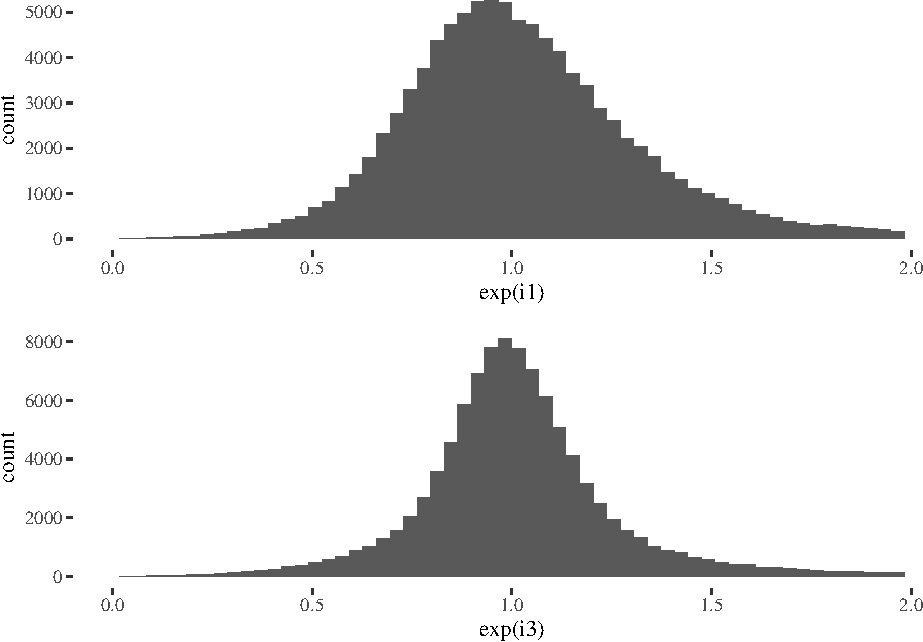
\includegraphics[width=1\linewidth]{ figures/priori1plot-1} \end{center}
\caption{Simulated priors for the individual i1 coefficients, and prior for the cumulative impact model with larger input variability (hence, the prior is more narrow to eliminate unrealistically huge impact).}
\label{fig:priori1plot}
\end{figure}



\section{Model choice for the long term analysis}\label{sec:priors}


let us elaborate on how we decided to use to the seemingly fairly
complicated model we already described in the body of the paper. Once preliminary causal considerations guided our
restrictions on variable selection, we proceed by building models of
increasing complexity, and comparing them in terms of Widely Acceptable
Information Criterion (which we have already discussed). The models
differ mostly in the underlying linear formulae. For computational ease
we will here use quadratic approximations, while in the final analysis
we will deploy Hamiltionian Monte Carlo. The names are meant to decode
the model structure: the predictors are listed before dashes, whereas
interactions are listed after dashes. The comparison results are in
Table \ref{tab:comparison} and plotted in Figure
\ref{fig:modelComparisonPlot}. Notice that there are ways of building a
complicated models that do not result in improvement, as they rather
lead to expected performance lower than that of the null model.


\footnotesize

\begin{center}
\begin{tabular}{p{5cm}l}
Null & $\mu_i  = \alpha$\\
ADS & $ \mu_i  = \alpha + \beta_{\mathsf{ADS}}\times \mathsf{ADS}$\\
ADSIC & $ \mu_i  = \alpha + \beta_{\mathsf{ADS}}\times \mathsf{ADS} +    \beta_{\mathsf{IC}}\times \mathsf{IC}$\\
IT & $ \mu_i  = \beta_{\mathsf{group}[i]} $\\
ADSIT & $\mu_i  = \alpha + \beta_{\mathsf{ADS}}\times \mathsf{ADS} +  \beta_{\mathsf{group}[i]}$\\
ADSITIC & $\mu_i  = \alpha + \beta_{\mathsf{ADS}}\times \mathsf{ADS} +  \beta_{\mathsf{group}[i]} +    \beta_{\mathsf{IC}}\times \mathsf{IC}$\\
ADSITIC-ADSIC & $\mu_i  = \alpha + \beta_{\mathsf{ADS}}\times \mathsf{ADS} +  \beta_{\mathsf{group}[i]} +    \beta_{\mathsf{IC}}\times \mathsf{IC} + $\\
& $  +  \beta_{\mathsf{ADSIC}}\times \mathsf{ADS} \times \mathsf{IC}$\\
ADSITIC-ADSIC-ADSIT & $\mu_i  = \alpha + \beta_{\mathsf{ADS}}[\mathsf{group}_i]\times \mathsf{ADS} +  \beta_{\mathsf{group}[i]} + $ \\
& $  +  \beta_{\mathsf{IC}}\times \mathsf{IC} + \beta_{\mathsf{ADSIC}}\times \mathsf{ADS} \times \mathsf{IC}$\\
ADSIT-ADSIT  & $ \mu_i   = \alpha + \beta_{\mathsf{ADS}}[\mathsf{group}_i] \times
 \mathsf{ADS} + \beta_{\mathsf{group}[i]} $\\
ADSITIC-ADSIT-ITIC-ADSIC  & $ \mu_i   = \alpha  +  \beta_{\mathsf{ADS}}[\mathsf{group}_i] \times \mathsf{ADS} + \beta_{\mathsf{group}[i]} + $ \\ 
& $ + 
\beta_{\mathsf{IC}}[\mathsf{group}_i] \times \mathsf{IC}     + \beta_{\mathsf{ADSIC}}\times \mathsf{ADS} \times \mathsf{IC}$\\
ADSITICCBS-ITIC-ADSIC & $\mu_i   = \alpha  +  \beta_{\mathsf{ADS}}[\mathsf{group}_i] \times
 \mathsf{ADS}  + \beta_{\mathsf{group}[i]} + $ \\ 
 &$ +    \beta_{\mathsf{IC}}[\mathsf{group}_i] \times \mathsf{IC}    + \beta_{\mathsf{CBS}} \times \mathsf{CBS} +  \beta_{\mathsf{ADSIC}}\times \mathsf{ADS} \times \mathsf{IC}$  \\
Final & $\mu_i  = \alpha + \beta_{\mathsf{ADS}}[\mathsf{group}_i]\times \mathsf{ADS} + \beta_{\mathsf{group}_i}  +  $ \\ & $ +  \beta_{\mathsf{IC}}[\mathsf{group}_i]\times \mathsf{IC} + $\\
&  $ + \beta_{\mathsf{ADSIC}}\times \mathsf{ADS} \times \mathsf{IC} + \beta_{\mathsf{CBS}}[\mathsf{group}_i] \times \mathsf{CBS} \nonumber$\\
tooFar & $\mu_i  = \alpha + \beta_{\mathsf{ADS}}[\mathsf{group}_i]\times \mathsf{ADS} + $ \\ & $ +  \beta_{\mathsf{group}_i}  +  \beta_{\mathsf{IC}}[\mathsf{group}_i]\times \mathsf{IC} +$ \\
 & $ + \beta_{\mathsf{ADSIC}}\times \mathsf{ADS} \times \mathsf{IC} + $ \\ & $ +  \beta_{\mathsf{CBS}}[\mathsf{group}_i] \times \mathsf{CBS} + \beta_{\mathsf{CBSIC}}\times
  \mathsf{CBS} \times \mathsf{IC} \nonumber$ 
\end{tabular}
\end{center}

\normalsize 


\footnotesize

\begin{table}
\centering\begingroup\fontsize{9}{11}\selectfont
\begin{tabular}{lrrrrrr}
\toprule
  & WAIC & SE & dWAIC & dSE & pWAIC & weight\\
\midrule
\cellcolor{gray!6}{Final} & \cellcolor{gray!6}{1184.829} & \cellcolor{gray!6}{89.779} & \cellcolor{gray!6}{0.000} & \cellcolor{gray!6}{NA} & \cellcolor{gray!6}{26.871} & \cellcolor{gray!6}{0.590}\\
tooFar & 1186.126 & 89.413 & 1.297 & 2.758 & 28.181 & 0.308\\
\cellcolor{gray!6}{ADSITICCBS\_ITIC\_ADSIC} & \cellcolor{gray!6}{1188.337} & \cellcolor{gray!6}{87.058} & \cellcolor{gray!6}{3.508} & \cellcolor{gray!6}{6.184} & \cellcolor{gray!6}{24.822} & \cellcolor{gray!6}{0.102}\\
IT & 1345.087 & 144.443 & 160.259 & 132.802 & 18.104 & 0.000\\
\cellcolor{gray!6}{null} & \cellcolor{gray!6}{1345.550} & \cellcolor{gray!6}{145.960} & \cellcolor{gray!6}{160.721} & \cellcolor{gray!6}{134.243} & \cellcolor{gray!6}{18.616} & \cellcolor{gray!6}{0.000}\\
ADS & 1348.696 & 143.821 & 163.867 & 132.558 & 22.718 & 0.000\\
\cellcolor{gray!6}{ADSITIC\_ADSIC} & \cellcolor{gray!6}{1351.556} & \cellcolor{gray!6}{152.861} & \cellcolor{gray!6}{166.728} & \cellcolor{gray!6}{139.154} & \cellcolor{gray!6}{29.070} & \cellcolor{gray!6}{0.000}\\
ADSIT & 1351.646 & 145.161 & 166.817 & 133.795 & 25.032 & 0.000\\
\cellcolor{gray!6}{ADSITIC} & \cellcolor{gray!6}{1352.087} & \cellcolor{gray!6}{146.835} & \cellcolor{gray!6}{167.258} & \cellcolor{gray!6}{134.608} & \cellcolor{gray!6}{27.254} & \cellcolor{gray!6}{0.000}\\
ADSIT\_ADSIT & 1352.672 & 155.862 & 167.844 & 142.092 & 31.855 & 0.000\\
\cellcolor{gray!6}{ADSIC} & \cellcolor{gray!6}{1352.892} & \cellcolor{gray!6}{146.359} & \cellcolor{gray!6}{168.064} & \cellcolor{gray!6}{134.313} & \cellcolor{gray!6}{26.421} & \cellcolor{gray!6}{0.000}\\
ADSITIC\_ADSIC\_ADSIT & 1355.482 & 155.522 & 170.653 & 141.405 & 33.558 & 0.000\\
\cellcolor{gray!6}{ADSITIC\_ADSIT\_ITIC\_ADSIC} & \cellcolor{gray!6}{1355.783} & \cellcolor{gray!6}{155.273} & \cellcolor{gray!6}{170.954} & \cellcolor{gray!6}{141.128} & \cellcolor{gray!6}{33.771} & \cellcolor{gray!6}{0.000}\\
\bottomrule
\end{tabular}
\endgroup{}
\caption{Model comparison results.}
\label{tab:comparison}
\end{table}

\normalsize 


\begin{figure}

\begin{center}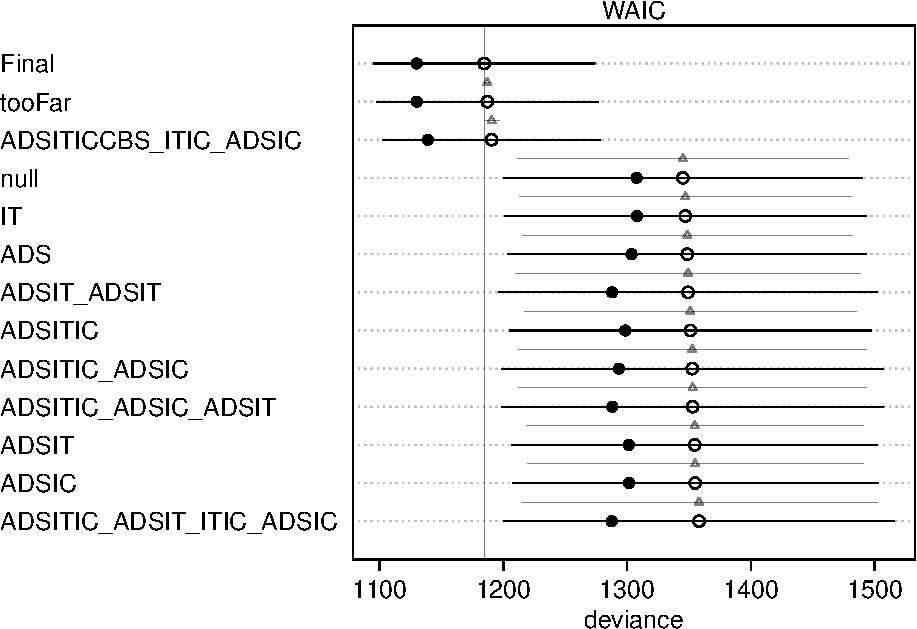
\includegraphics[width=1\linewidth]{ figures/fig:modelComparison-1} \end{center}
\caption{Model comparison, WAIC scores. The filled points are the in-sample deviance values. The open points are the WAIC values. The line segments represent standard errors of the WAIC scores. really want however is the standard error of the difference in WAIC
between the two models. The triangle is the difference to the top rated model, and the line segment going through it is the standard error of this difference.}
\label{fig:modelComparisonPlot}
\end{figure}





The three models that stand out differ in including \(\mathsf{CBS}\) as
a predictor. Moreover the final model includes an interaction between
treatment group and \(\mathsf{CBS}\). Adding a further interaction
between \(\mathsf{CBS}\) and \(\mathsf{IC}\) takes us too far. We will
employ the top model (\(\mathsf{Final}\)) in further analyses.





Now, to sensibly set up our priors, let's  build two models with the general structure reached. One with fairly
wide priors that one might initially think are appropriate, one with
regularizing priors. The key phenomenon to watch out for in such
contexts (slightly complex models with interactions) is that it is hard
to intuitively predict the impact of coefficient priors on prior
predictions. For this reason, we run prior predictive checks for both
models, and we select the priors that do not result in unrealistically wide prior predictions. 




\begin{figure}

\begin{center}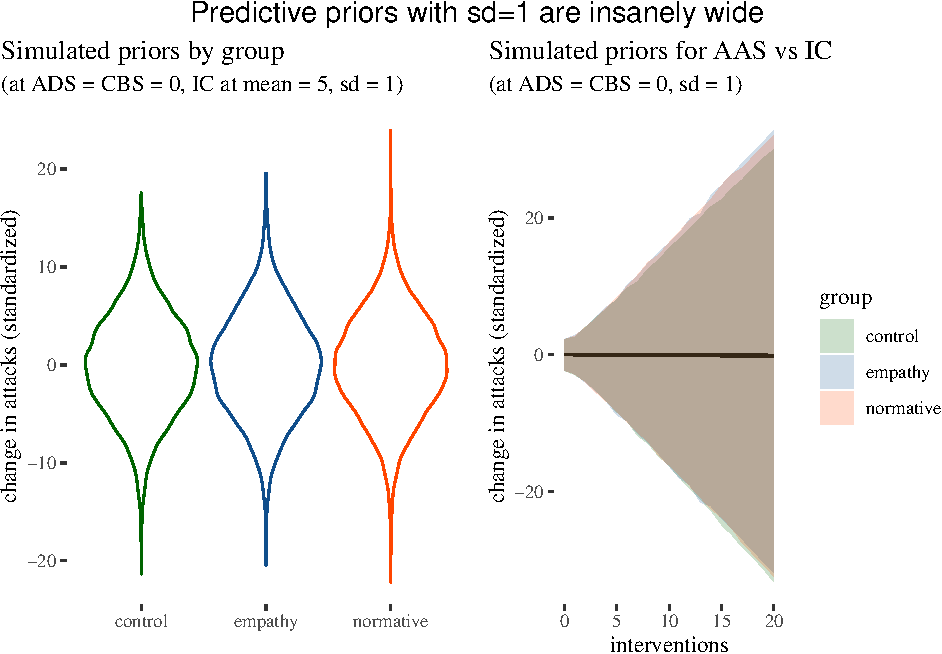
\includegraphics[width=0.8\linewidth]{ figures/fig:priorCheck-1} 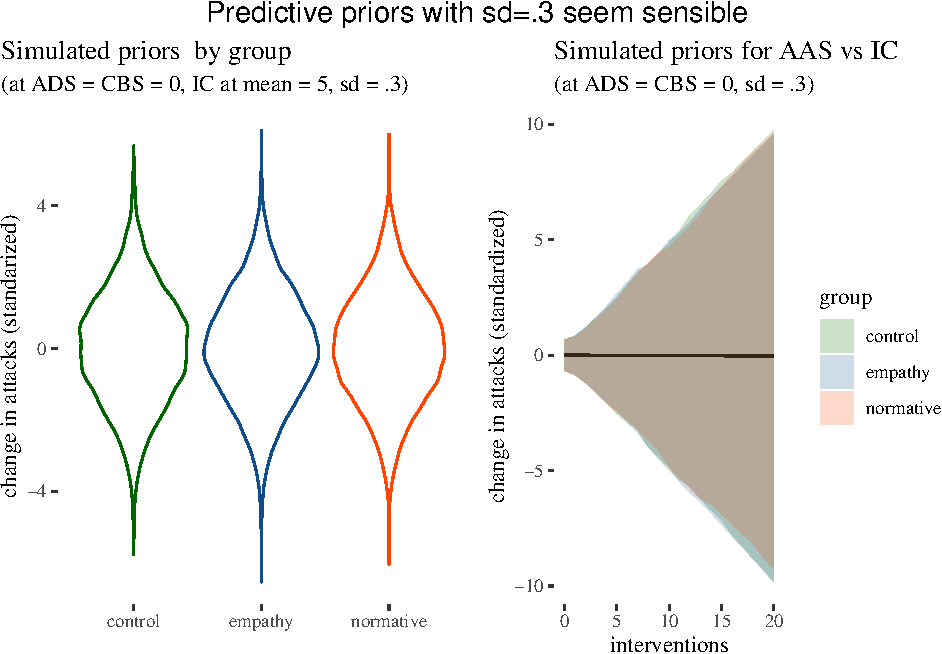
\includegraphics[width=0.8\linewidth]{ figures/fig:priorCheck-2} \end{center}

\caption{Prior predictive check for two different sets of priors.}
\label{fig:priors}
\end{figure}














%% \section{}
%% \label{}

%% For citations use: 
%%       \citet{<label>} ==> Jones et al. [21]
%%       \citep{<label>} ==> [21]
%%

%% If you have bibdatabase file and want bibtex to generate the
%% bibitems, please use
%%

%% else use the following coding to input the bibitems directly in the
%% TeX file.

%%\begin{thebibliography}{00}

%% \bibitem[Author(year)]{label}
%% Text of bibliographic item

%%\bibitem[ ()]{}

%%\end{thebibliography}

%\bibliographystyle{elsarticle-num-names}
%\bibliography{attacks}

\end{document}

\endinput
%%
%% End of file `elsarticle-template-num-names.tex'.
